\documentclass[10pt, aspectratio=169]{beamer}
\usepackage{appendixnumberbeamer}
\usepackage{siunitx}
\usepackage[utf8]{inputenc} \usepackage[T1]{fontenc}
\usepackage{booktabs} \usepackage[scale=2]{ccicons}
\usepackage[backend=biber]{biblatex}
\usepackage{stackengine}
\usepackage[version=4]{mhchem}
\usepackage{physics}
\usepackage{pgfpages}
\usepackage{multimedia}
\usepackage{lmodern}
\setbeameroption{show notes on second screen} %
% \setbeamercovered{transparent}
\addbibresource{slides.bib}
\graphicspath{ {figs/} }

\usetheme{Antibes}
\setbeamertemplate{itemize items}[default]
\setbeamertemplate{enumerate items}[default]
\AtBeginSection[]
{
   \begin{frame}
       \tableofcontents[currentsection]
   \end{frame}
}
\setbeamertemplate{footline}[frame number]

\setbeamertemplate{note page}[plain]
% \usepackage[font={scriptsize,it}]{caption}
\usepackage{hyperref}
\sisetup{prespace}
\newcommand{\laser}{\textsc{Laser}}
\newcommand{\hne}{\ce{HeNe}}
\sisetup{separate-uncertainty = true}

\title{Gaslaser}
\subtitle{Total Laser!}
\author{Valentin Boettcher}
\beamertemplatenavigationsymbolsempty

\begin{document}
\hypersetup{pageanchor=false}
\maketitle

\hypersetup{pageanchor=true}
\pagenumbering{arabic}
\begin{frame}
  \tableofcontents
\end{frame}

\section{Allgemeines zum Versuch}

\begin{frame}{Mit Laser und so...}
  \begin{block}{Acronym}
    \textsc{Light Amplification by Stimulated Emission of Radiation.}
  \end{block}

  \pause

  \begin{block}{Basic Facts}
    \pause
    \begin{itemize}
    \item erster Laser um 1960 von Theodore H. Maiman
      \begin{itemize}
      \item bezeichnet als ``L\"osung auf der Suche nach einem
        Problem''~\cite{2010}
      \end{itemize}
      \pause
    \item kann sehr \textbf{fokussiertes}, \textbf{koh\"arentes} und
      \textbf{intesives} Licht erzeugen \pause
    \item findet Anwendung in breiten Bereichen der Technik und
      Wissenschaft
      \begin{itemize}
      \item Barcode Scanner, CD-Spieler, Optische
        Telekommunikationstechnik \pause
      \item Erzeugung tiefer Temperaturen, Schockwellen, gro\ss{}en
        Energiedichten, Holographie, Interferometrie,
        Teilchenbeschleuniger
      \end{itemize}
    \end{itemize}
  \end{block}
\end{frame}

{
  \usebackgroundtemplate{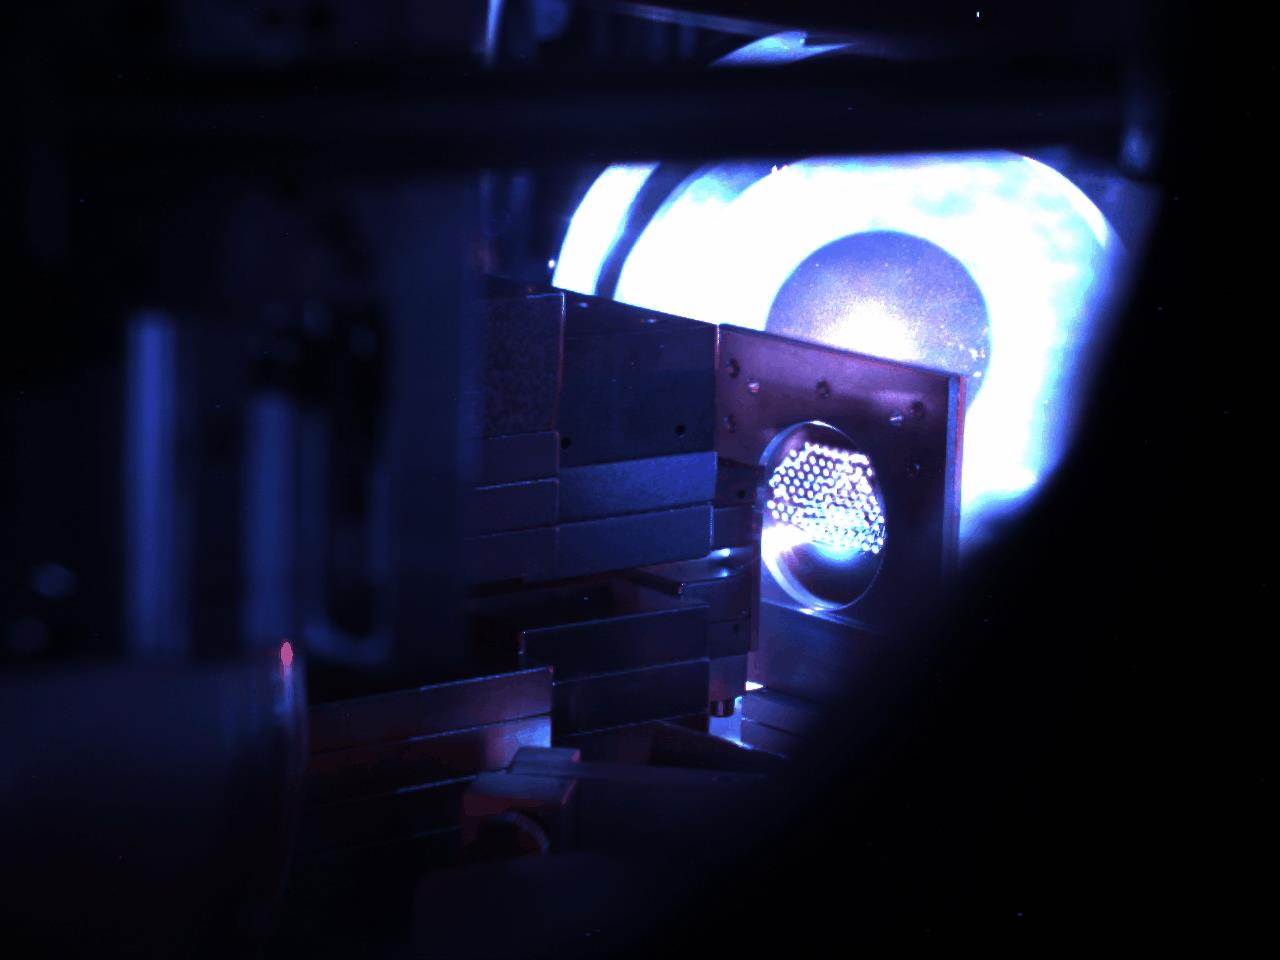
\includegraphics[width=\paperwidth]{propaganda.png}}
  \begin{frame}[plain]
    \note[item]{kurz was zu laser teilchenbeschleuniger,  (3µm Durchmesser, Intensität beträgt ~$10^21 Watt/cm^2$}


  \end{frame} % sthn
}

\begin{frame}{Versuchsziel und Aufbau}
  \begin{columns}
    \column{.5\textwidth}
    \begin{figure}[H]
      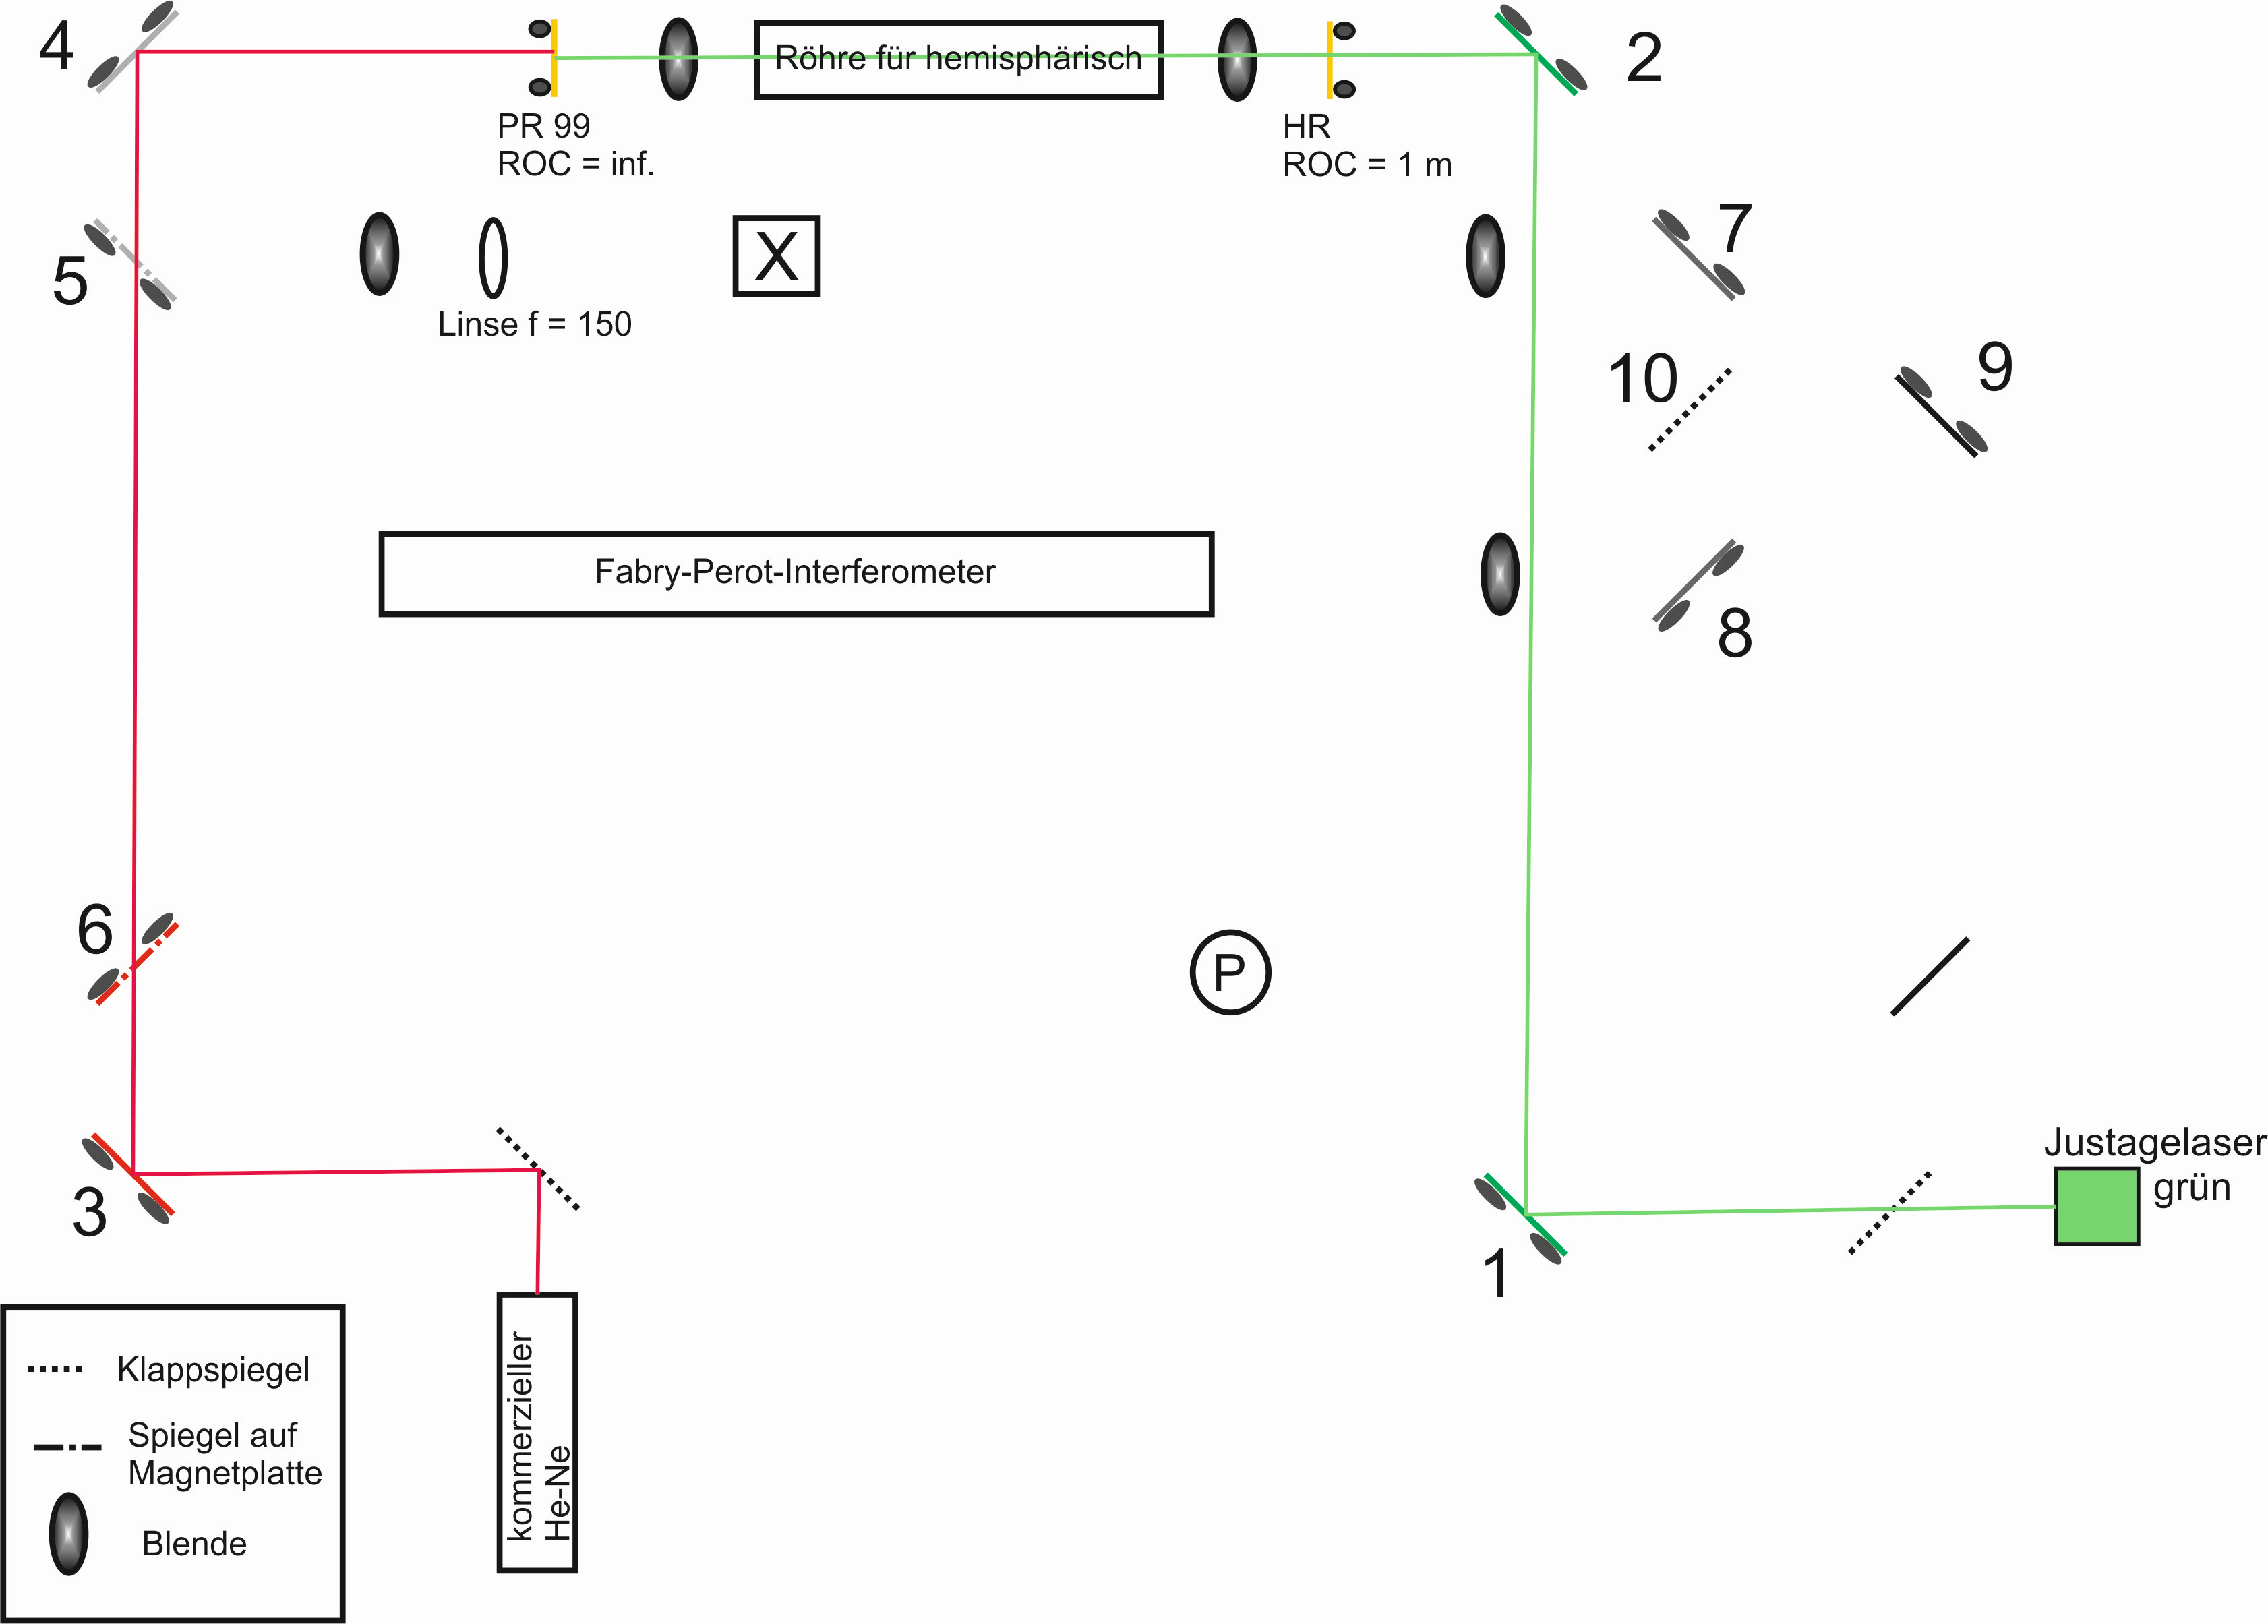
\includegraphics[width=1\columnwidth]{aufb.png}
    \end{figure}
    \column{.5\textwidth} \uncover<1,2>{
      \begin{block}{Ziel des Versuches}
        Justierung, Inbetriebnahme und Untersuchung eines \hne{} Lasers.
      \end{block}
    } \uncover<2>{
      \begin{block}{Zur Verf\"ugung stehendes Material}
        \begin{description}
          \item[Optische Komponenten] Spiegel, Blenden, Linsen,
            Plofilter
          \item[Laser] kommerzieller \hne{} und gr\"uner Justagelaser
          \item[Laserr\"ohre] \hne{} Entladungsr\"ohre
          \item[Leistungsmessger\"at] Zur Leistungsmessung und als
            Justagehilfe.
        \end{description}
      \end{block}
    }
  \end{columns}
\end{frame}


\section{Aufbau und Theorie des Lasers}
\subsection{Grundlegender Aufbau und Funktionsweise eines Lasers}
\label{sec:funkt}
\begin{frame}
  \begin{columns}
    \column{.5\textwidth}
    \begin{figure}[H]\centering
      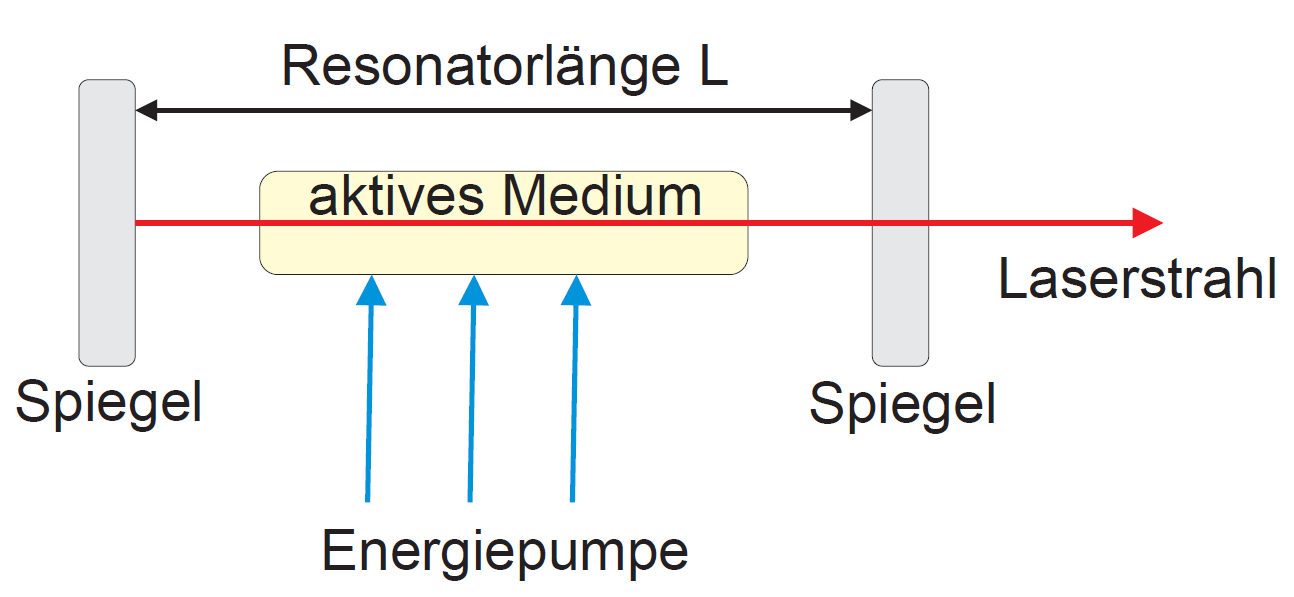
\includegraphics[width=\columnwidth]{schema.png}
    \end{figure}

    \column{0.5\textwidth}
    \begin{block}{Aufbau}
      \begin{itemize}
      \item Akives Medium
        \begin{itemize}
        \item Gase Festk\"orper
        \end{itemize}
      \item Optischer Resonator
        \begin{itemize}
        \item meist rotationssymmetrische, sph\"arische Spiegel
        \end{itemize}
      \item Energiepumpe
        \begin{itemize}
        \item Lichtblitze, Elektronenst\"oße
        \end{itemize}
      \end{itemize}
    \end{block}
  \end{columns}
\end{frame}

\begin{frame}{Funktionsweise}
  \begin{block}{Acronym}
    \textsc{Light Amplification by Stimulated Emission of Radiation.}
  \end{block}

  \begin{enumerate}
  \item<1-> Energiepumpe erzeugt Ungleichgewichtsbesetzung von
    Energieniveaus im aktiven Medium
  \item<2-> Photonen oszillieren im Resonator mehrfach, werden bei
    jedem Durchlauf verst\"arkt \(\implies\)
  \item<3-> Bruchteil des Lichtes wird ausgekoppelt und genutzt
  \end{enumerate}
\end{frame}

\subsection{Besetzungsinversion und Laserbedingungungen}
\begin{frame}
  \begin{itemize}
  \item betrachte ein Zweiniveausystem \(1,2\), Besetzungszahlen
    \(N_1, N_2\)
  \item f\"ur elektromagnetische atomare \"Uberg\"ange gilt:
    \begin{equation}
      h\nu = E_2 - E_1
    \end{equation}
  \end{itemize}
  \pause
  \begin{block}{Absorbtions und Emissionsprozesse}
    \begin{description}
    \item<2->[Absorption] Absorption eines Photons wird von Atom
      absorbiert, Anregung \(1\rightarrow 2\)
      \note<2>[item]{H\"aufigkeit proportional zu spektraler
        Energiedichte}
    \item<3->[Spontane Emission] Aussendung eines Photons, Spontane
      Abregung des Atoms \(2\rightarrow 1\)\note<3>[item]{unabh\"angig
        von der umgebenden spektralen Energiedichte}

    \item<4->[Stimulierte Emission] Photon mit passender
      Energie\note<4>[item]{siehe obige Formel} stimuliert angeregtes
      Atom zur Abregung \(2\rightarrow 1\), Aussendung eines identischen
      Photons\note<4>[item]{Phase, Polar. etc}
      \note<4>[item]{H\"aufigkeit dieses Prozesses ist proportional
        zur spektralen Energiedichte.}
    \end{description}
  \end{block}
\end{frame}


\begin{frame}{Besetzungsinversion}
  \begin{itemize}
  \item<1-> im thermischen Gleichgewicht \"uberwiegt die spontane
    Emission gegen\"uber der Induzierten \(\implies\) Erzeugung eines
    Ungleichgewichts durch ``Pumpen'' \note<1->[item]{im folgenden
      Spontane Emission vernachl\"assigt, erzeugt aber neue Moden,
      siehe sp\"ater, konzentriert man verst\"arkung auf best. Moden
      \"uberwiegt stim e}\note<1->[item]{ Negative Temp}
  \item<2-> Ratengleichung f\"ur Photonenzahl\note<2->[item]{Modell der Einsteinkoeffizienten, als
      Bedingung der Verst\"arkung} ergibt:
    \begin{equation}
      \label{eq:firstlaser}\tag{Erste Laserbedingung}
      N_2>N_1
    \end{equation}
    \(\implies\) Besetzungsinversion
  \item<3-> Zweite Laserbedingung: Verst\"arkung \(>\) D\"ampfung
    \note<3->[item]{Definiert Verlustgrenze}

    \note<2->[item]{Besetzungsinversion ist erst mit Vierniveausystem
    realisierbar (metastabile Zust\"ande halten Grundzustand
    lehr),sonst grosse Pumpleistung notwendig, 2 da
      pumpen mit emission konkurriert, 3 da unteres Niveau
      Grundzustand, vierniveau hat niveau unter unterem laser niv,
      pumpen an laser\"ubergang vorbei}
  \end{itemize}
\end{frame}

\begin{frame}{\hne{} System}
  \begin{columns}
    \column{.5\textwidth}
    \begin{figure}[H]
      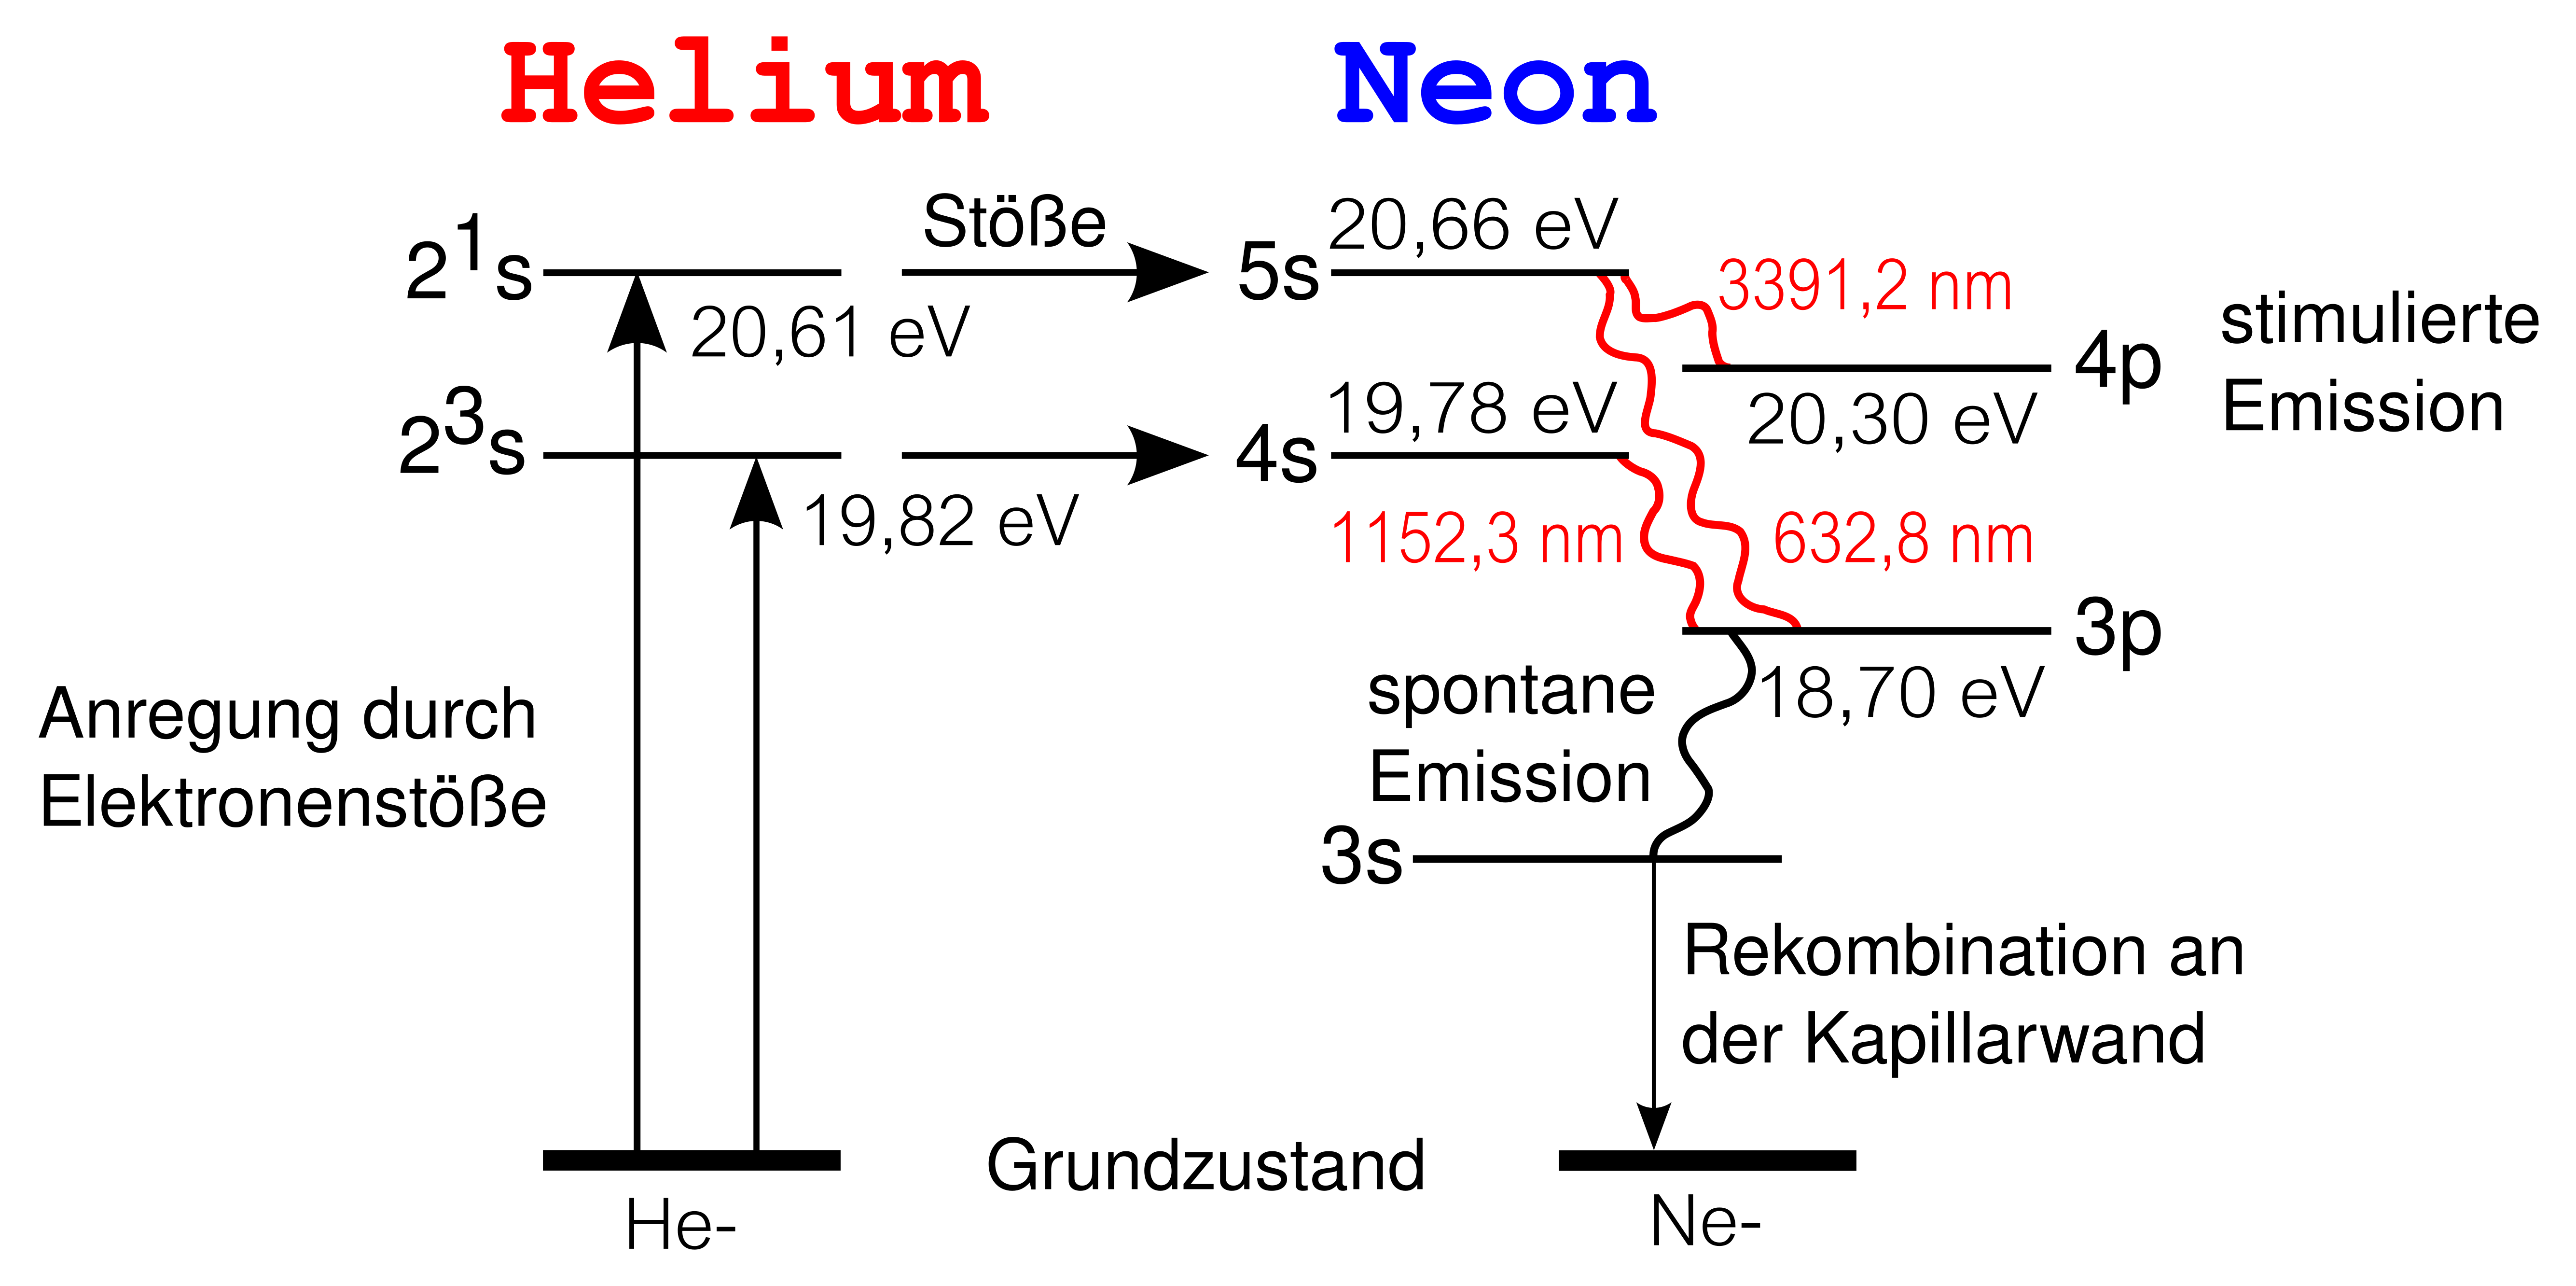
\includegraphics[width=1\columnwidth]{heneniv.png}
    \end{figure}
    \column{.5\textwidth}
    \begin{itemize}
    \item<1-> Pumpen von Helium durch Elektronensto\ss{}
    \item<2-> Helium regt durch St\"o\ss{}e \"anlich gelegene Niveaus
      im Neon an (Zufall)
    \item<3-> Nutzung des \"Ubergangs \(5S\rightarrow 3P\) (sichtbar)
    \item<4-> Lebensdauer des \(P\) Niveaus ausreichend kurz
    \end{itemize}
  \end{columns}
\end{frame}

\subsection{Justage und Messung der Verst\"arkung im
  Einfachdurchgang}
\begin{frame}{Einfachverst\"arker \(\neq\) Laser}
  \begin{itemize}
  \item<1-> Justage der beiden Justagelaser parallel zur Optischen
    Achse (OA) der \hne{}-R\"ohre \note<1->[item]{Ein wenig zur
      technik...}\note<1->[item]{Reflexe an Kapillarw\"anden}
  \item<2-> Untersuchung des Verst\"arkungseffektes im
    Einfachdurchgang mithilfe eines kommerziellen \hne{} Lasers
    \(\implies\) Messung der Leistung vor und Nach der R\"ohre
  \end{itemize}

  \uncover<3->{
    \begin{table}
      \begin{tabular}{l|SSSS}
        \toprule
        & {Mittelwert [\si{\micro\watt}]} & {\(\sigma\)
                                            [\si{\micro\watt}]} & {Minimum
                                                                  [\si{\micro\watt}]}
        & {Maximum [\si{\micro\watt}]} \\
        \midrule
        Untergrund & 0.839 & 0.031 & 0.771 & 0.888 \\
        R\"ohre aktiv & 965.161  & 4.2  & 958.229  & 973.112  \\
        R\"ohre inaktiv & 907.161  & 17.5 & 885.229  & 949.112  \\
        vor R\"ohre & 1319.161 & 2.0  & 1319.229 & 1329.112 \\
        \bottomrule
      \end{tabular}
      \caption{Leistungsmessung des Einfachdurchgangs mit
        abgezogenem Untergrund}
    \end{table}}
  \begin{itemize}
  \item<4-> Untergrund ist Vernachl\"assigbar
  \item<5-> aktive R\"ohre verst\"arkt nur um \SI{6}{\percent}
  \end{itemize}
  \note<3->[item]{Messzeit \SI{150}{\second} festgelegt, da
        Schwankung cons.}
  \note<4->[item]{zu wenig zeit f\"ur noch laenger}
  \note<5->[item]{Syst. vernachl. fehler aus stat}
  \note<5->[item]{Notwendigkeit Resonator}
\end{frame}

\subsection{Optischer Resonator}
\label{sec:reso}

\begin{frame}{Optischer Resonator}
  \begin{columns}
    \column{.5\textwidth} \only<2->{
      \begin{figure}
        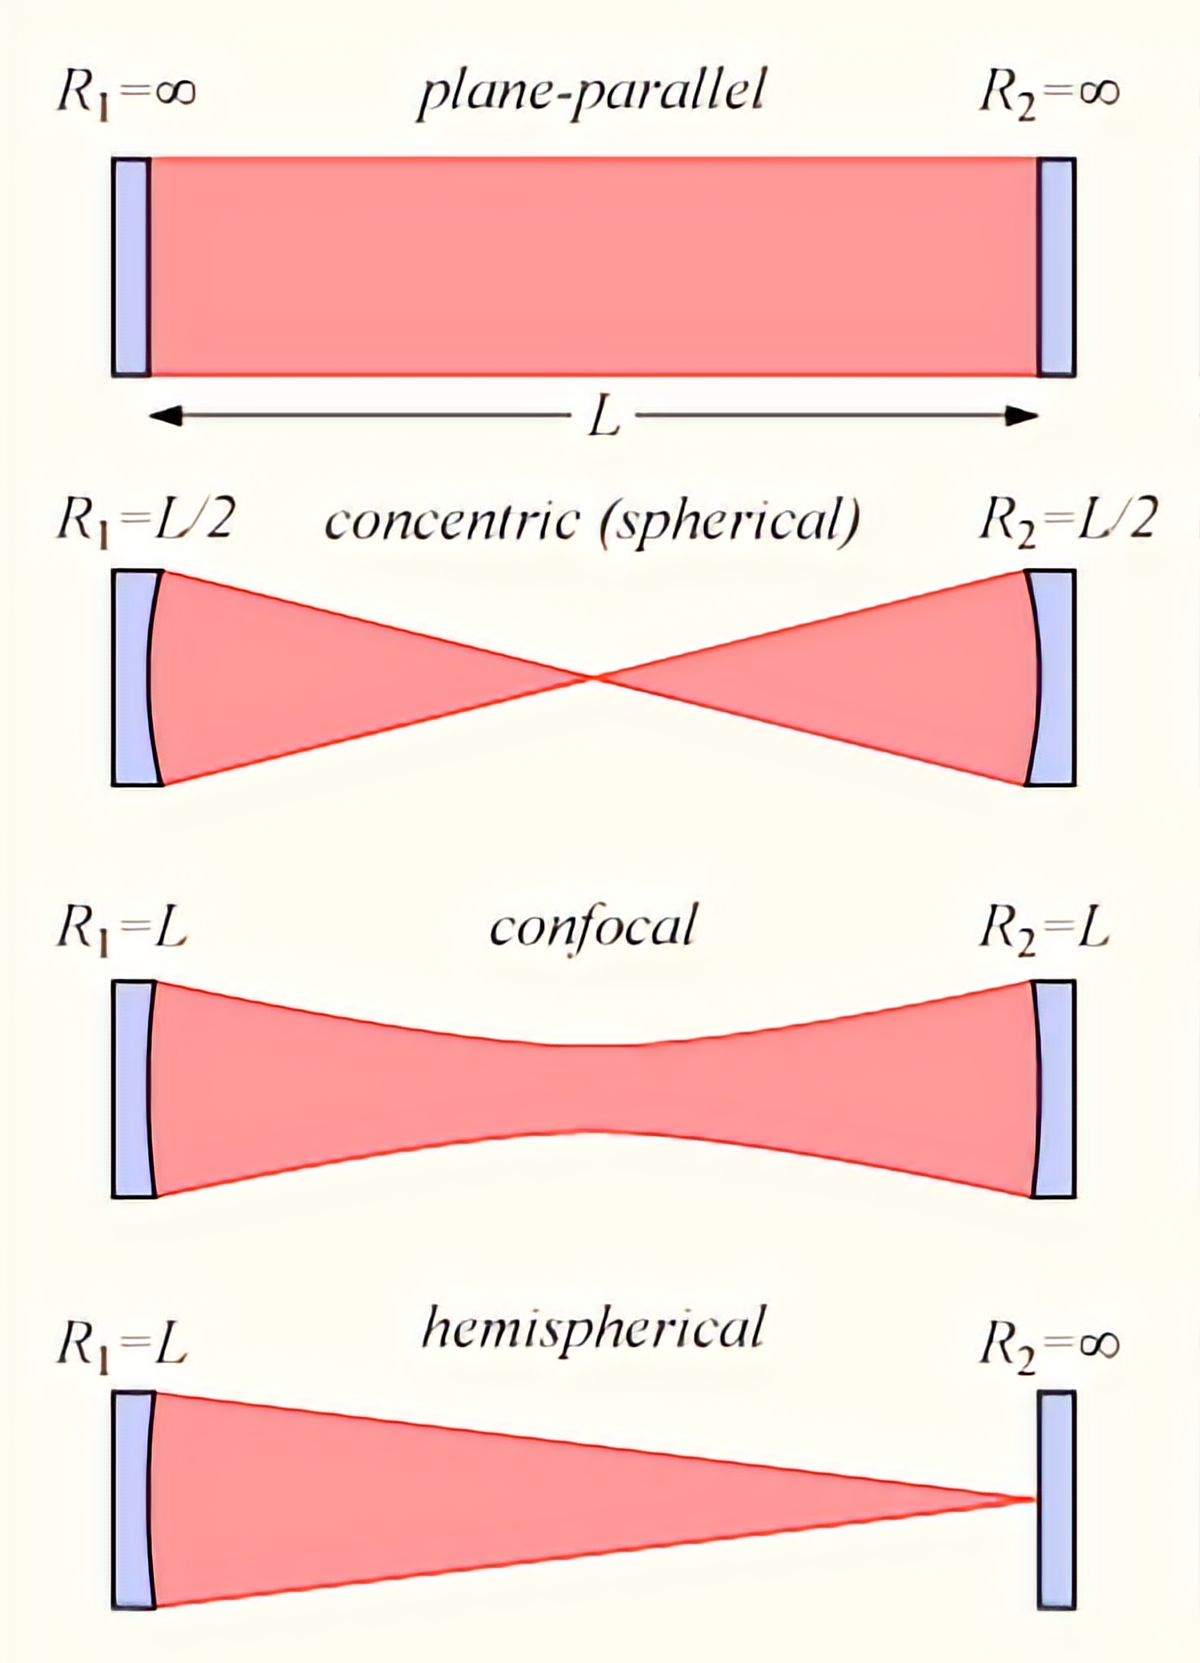
\includegraphics[width=.6\columnwidth]{Optical-cavity1.png}
      \end{figure}
    } \column{.5\textwidth}
    \begin{itemize}
    \item<1-> Erzeugung eines stabilen Strahlungsfeldes durch
      oftmalige Reflexion
    \item<2-> oft durch zwei Spiegel realisiert
    \item<2-> in diesem Versuch: hemisph\"arische Konfiguration
    \end{itemize}
  \end{columns}
\end{frame}

\begin{frame}{Resonanz und Modenstruktur}
  \begin{columns}
    \column{.5\textwidth} \only<3->{
      \begin{figure}
        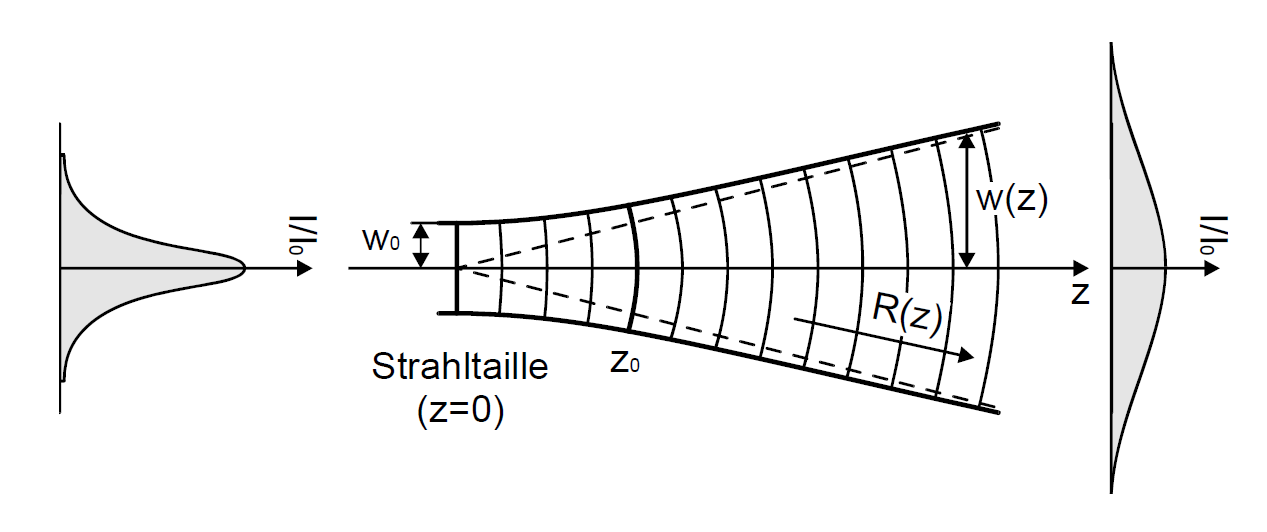
\includegraphics[width=1\columnwidth]{gauss-strahl.png}
      \end{figure}
    } \column{.5\textwidth}
    \begin{itemize}
    \item<1-> longitudinale Resonanzbedingung:\note<1->[item]{stehende
        Welle, in realit\"at nur ein paar Moden ausgeprägt,
        Modenkonkurrenz}
      \begin{equation}
        \label{eq:longmodes}
        L=n\cdot\frac{\lambda}{2} \implies \Delta\nu = \frac{c}{2L}
      \end{equation}
    \item<2-> Beschreibung des gesamten Feldes durch paraxiale
      L\"osung der Maxwellgleichungen \note<2->[item]{Vakuum,
        anpassen der RB an Spiegel Radien}
    \item<3-> ergibt als Grundmode sog. \textbf{Gauss-Strahl}
      (Querschnitt ist Gaussfunktion) \note<3->[item]{h\"ohere Moden
        weiter aufgeweitet und leicht mit Blenden zu unterdr\"ucken}
    \end{itemize}
  \end{columns}
\end{frame}

\begin{frame}{Stabilit\"at im Resonator}
  \begin{columns}
    \column{.5\textwidth}
    \begin{figure}
      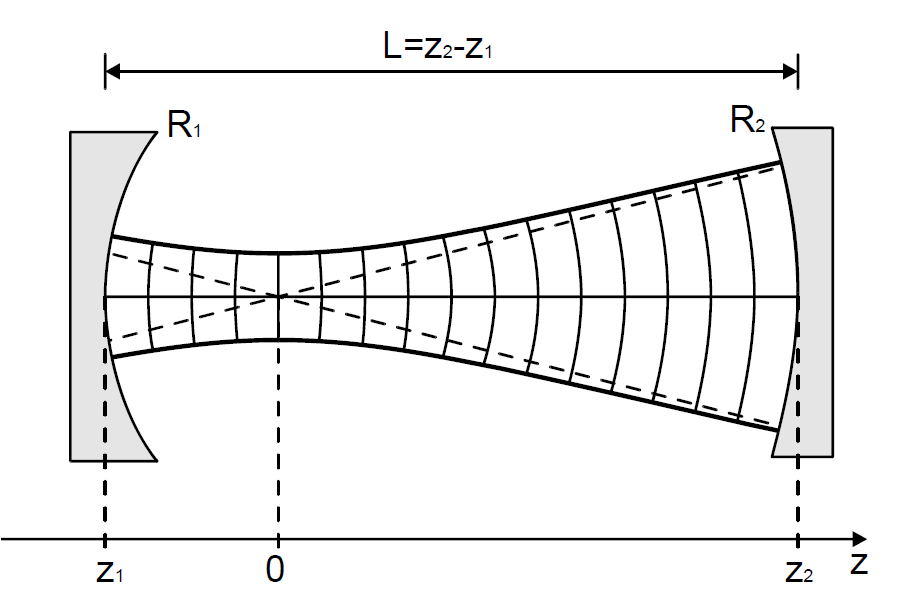
\includegraphics[width=1\columnwidth]{gauss-res.png}
    \end{figure}
    \column{.5\textwidth}
    \begin{itemize}
    \item<1-> Passe Gausstrahl so an, dass
      \(R(z_1)=R_1,\; R(z_2)=R_2\), definiere:
      \begin{equation}
        \label{eq:gparams}
        g_i=1-\frac{L}{R_i};\; i=1,2
      \end{equation}
    \item<2-> es folgt durch Anpassen der L\"osung dass Resonator
      stabil falls:\note<1->[item]{keine Matrizenoptik}
      \begin{equation}
        \label{eq:stabbed}
        0\leq g_1g_2\leq 1
      \end{equation}
    \end{itemize}
  \end{columns}
\end{frame}


\subsection{Berechnung des Stabilit\"atsbereichs}
\label{sec:stab}

\begin{frame}
  Da \(g_1(R_1=\infty)=1\) folgt mit
  \(R_2=\SI{1}{\meter}\) und \(0\leq g_2\leq 1\)
  durch~\ref{eq:stabbed}:

  \begin{equation}
    \label{eq:stabber}
    g_2=1-\frac{L}{\SI{1}{\meter}}\implies\SI{0}{\meter}\leq L \leq \SI{1}{\meter}
  \end{equation}

  \begin{figure}[H]\centering
    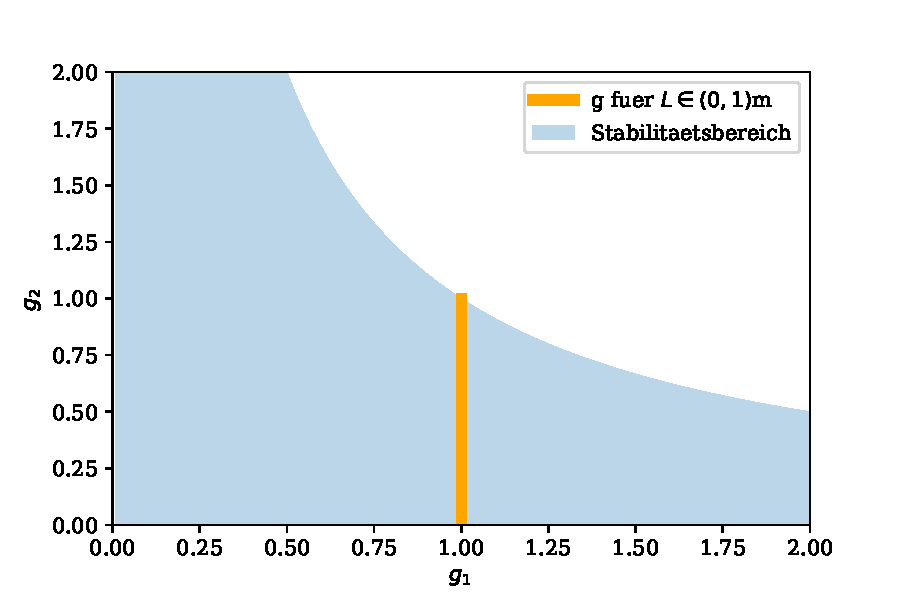
\includegraphics[width=.5\columnwidth]{figs/stabdiag.pdf}
  \end{figure}
\end{frame}


\subsection{Aufbau des Hemisph\"arischen Resonators}
\begin{frame}{Laser, Marke: Eigenbau}
  \begin{itemize}
  \item<1-> Einbau der Resonatorspiegel (planar und sph\"arisch)
  \item<2-> Justage mittels R\"uckreflexen
  \item<3-> Feinjustage durch Beamwalken (iteratives Feinjustieren der
    Stellschrauben an den Spiegel) \(\implies\) Maximalleistung auf
    \SI{1}{\milli\watt}
  \item<4-> Variation der Resonatorl\"ange und Leistungsmessung
    \begin{itemize}
    \item Ableseschwierigkeiten ergeben eine gesch\"atzte Unsicherheit
      \(\Delta L = \SI{.5}{\centi\meter}\)
    \end{itemize}
  \end{itemize}

  \note<4->[item]{Jeweils leistungsmaximierung durch Beamwalk}
\end{frame}

\begin{frame}
  \begin{figure}[H]\centering
    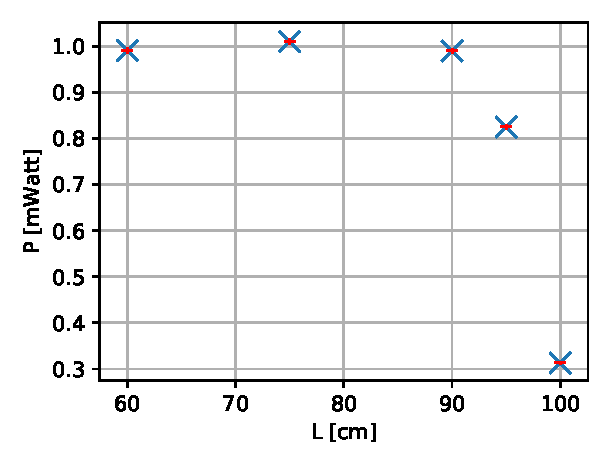
\includegraphics[width=.5\columnwidth]{figs/power-over-l.pdf}
  \end{figure}
  \begin{itemize}
  \item<1-> Leistungseinbruch bei \SI{1}{\meter} deutlich zu erkennen
  \item<2-> Fr\"uhes Einsetzen des Einbruch:
    \begin{itemize}
    \item zunehmende Ung\"ultigkeit der paraxialen N\"aherung
    \item Justage empfindlicher: Leistungsmaximum nicht gefunden
    \end{itemize}
  \item<3-> Festlegung \(L=\SI{80}{\centi\meter}\)
  \end{itemize}
\end{frame}

\section{Strahleigenschaften der Grundmode}
\label{sec:seig}

\subsection{Matrizenoptik}
\label{sec:mao}


\begin{frame}
  \begin{columns}
    \column{.5\textwidth}
    \begin{figure}
      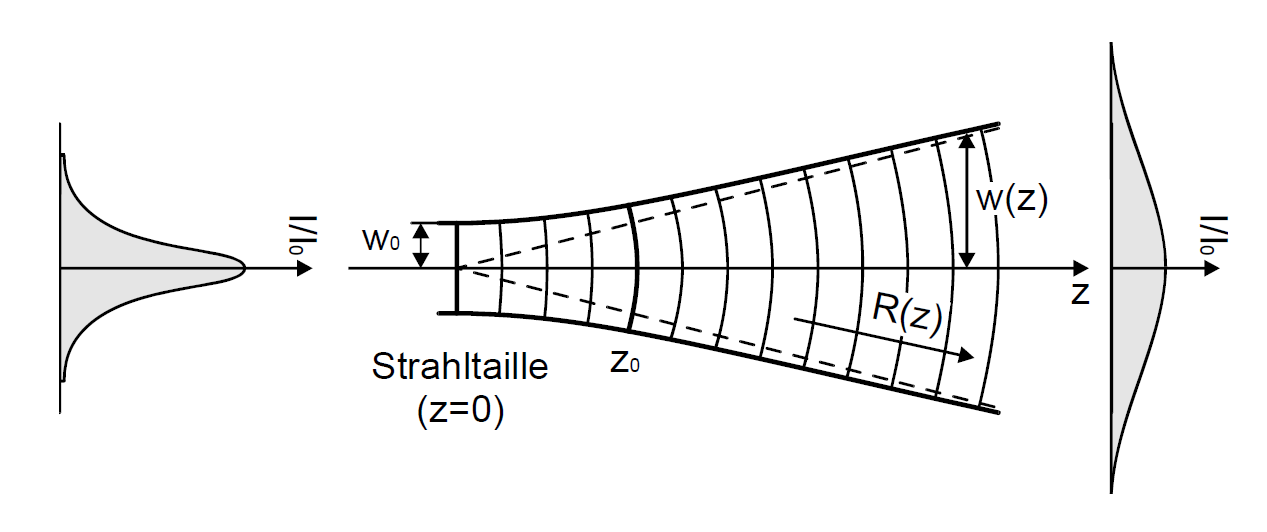
\includegraphics[width=1\columnwidth]{gauss-strahl.png}
    \end{figure}
    \begin{align*}
      \label{eq:gauss}
      \displaystyle E(r,z)&=E_{0}\;{\frac {w_{0}}{w(z)}}\cdot \mathrm
                            {e} ^{-\left({\frac {r}{w(z)}}\right)^{2}}\cdot \mathrm {e}
                            ^{-ik{\frac {r^{2}}{2R(z)}}}\cdot \mathrm {e} ^{-i(kz-\zeta
                            (z))} \\
                          &= \ldots \mathrm{e}^{-r^2 \frac{\pi}{\lambda}i\cdot q}\ldots
    \end{align*}
    \column{.5\textwidth}
    \begin{block}{Gauss-Strahl, Revisited}
      \begin{itemize}
      \item charakterisiert durch Strahldicke \(w(z)\), Radius der
        Wellenfronten \(R(z)\)
        \pause
      \item freihe Parameter: Amplitude, Strahltaille \(w(z=0)=w_0\),
        Polarisation und Wellenl\"ange
      \pause
    \item \(w(z)=w_0\cdot\sqrt{1+\qty( \frac{z\cdot\lambda}{\pi\cdot w_0^2})^2}\)
      \end{itemize}
    \end{block}

  \end{columns}
\end{frame}
\note[itemize]{
  \item \(\zeta\) ist Gouy Phase, hier nicht so wichtig -> wird
    konstant
  \item radius \(R\) erst eben, steigt asympt linear genau wie waist
  \item \(z_0=\frac{\pi w_0^2}{\lambda}\) rayleigh
  }
\begin{frame}{Crashkurs Matrizenoptik}
  \begin{itemize}
  \item<1-> Annahmen: Paraxiale Optik, alle Winkel Klein
  \item<2-> stelle strahl als 2er Vektor da:
    \begin{equation}
      \mqty(d \\ \alpha) \widehat{=} \mqty(\text{Abstand zur Achse} \\
      \text{Winkel zur Achse})
    \end{equation}

  \item<3-> optisches System dargestellt druch Matrix als Produkt der
    Komponenten:
    \begin{gather}
      \label{eq:systmatrix}
      \mathfrak{M}_{\text{System}}=\mathfrak{M}_{\text{1}}\cdot\ldots\cdot\mathfrak{M}_{n}=\mqty(A
      & B \\ C & D) \\
      \mqty(d' \\ \alpha') = \mathfrak{M}_{\text{System}}\cdot\mqty(d
      \\ \alpha)
    \end{gather}
  \end{itemize}
\end{frame}
\begin{frame}{Einige Optische Komponenten}
  \begin{table}[h!]
    \begin{tabular}{l | c | l}
      \textbf{Element} & \textbf{Matrix} & \textbf{Parameter} \\
      \midrule\\
      \addlinespace[-2ex]
      freie Ausbreitung & \(\begin{pmatrix}
        1 & s \\
        0 & 1
      \end{pmatrix}\) & Wegl\"ange \(s\) \\
      \midrule\\
      \addlinespace[-2ex] d\"unne Linse & \(\begin{pmatrix}
        1 & 0 \\
        -1/f & 1
      \end{pmatrix}\) & Brennweite \(f\) \\
      \midrule\\
      \addlinespace[-2ex] sph\"arischer Spiegel & \(\begin{pmatrix}
        1 & 0 \\
        -2/R & 1
      \end{pmatrix}\) & Radius \(R\) \\

    \end{tabular}
  \end{table}
\end{frame}

\begin{frame}
  \begin{alertblock}{Achtung, High-Level}
    Sieht komisch aus ist aber so. \textbf{Matrizen als
      M\"obius Abbildungen.}\note<1->[item]{Urspr\"unge ein
      wenig erkl\"aren. Konforme Abbildung}
  \end{alertblock}

  \begin{itemize}
  \item<2-> definiere
    \(\frac{1}{q(z)}=\frac{1}{R(z)}-i\frac{\lambda}{\pi
      w^2(z)}=a+i\cdot b\) \note<2->[item]{ist exponent der e funktion
      in mathem. Darstellung Gausstrahl ERRINNERN}
  \item<3-> mit
    \(\mathfrak{M}_{\text{System}} = \mqty(A & B \\ C & D)\)
    transformiert sich \(q\) wie folgt:
    \begin{equation}
      \label{eq:qtrans}
      q'=\frac{Aq + B}{Cq+D}
    \end{equation}

    \item<4-> der Beamwaist des Austretenden strahls, verschoben zu Linse
      fokussiert durch Linse mit Brennweite (A,B,C,D entsprechend
      Tabelle):
      \begin{equation}
        \label{eq:qkaust}
        b'=b\cdot\frac{AD-CB}{A^2+B^2b^2}
      \end{equation}
      \begin{equation}
        \label{eq:reswaist}
        w'=\sqrt{\frac{\lambda}{\pi\cdot b'(x)}}
      \end{equation}
  \end{itemize}
\end{frame}

\subsection{Messung der Kaustik}
\begin{frame}
  \begin{columns}
    \column{.5\textwidth}
    \begin{itemize}
    \item<1-> Einbringen einer Linse mit \(f=\SI{15}{cm}\) im Abstand
      \(s=\SI{64.5\pm 2.0}{\centi\meter}\) in den Strahlengang
    \item<2-> Ausblendung der h\"oheren transversalen Moden
    \item<3-> Aufnehmen der Strahlkaustik\note<2->[item]{Tafel} mit
      CCD Kamera
      \begin{itemize}
      \item Anpassen der Belichtung sodass eine S\"attigung
        \(200/255\) erreicht wurde
      \item Bestimmung des FWHM mit Gauss-Fit durch Software
        \textsc{Laser Light Inspector} \note<3->[item]{tafel}
      \end{itemize}
    \item<4-> Unsicherheiten:
      \begin{itemize}
      \item \(\Delta s\) aus Ableseschwierigkeiten
      \item Aufl\"osung der Kamera
        \(\SI{1}{px}=\SI{5.6}{\micro\meter}\)
      \end{itemize}
    \end{itemize}
    \column{.5\textwidth} \only<1-5>{
      \movie[loop]{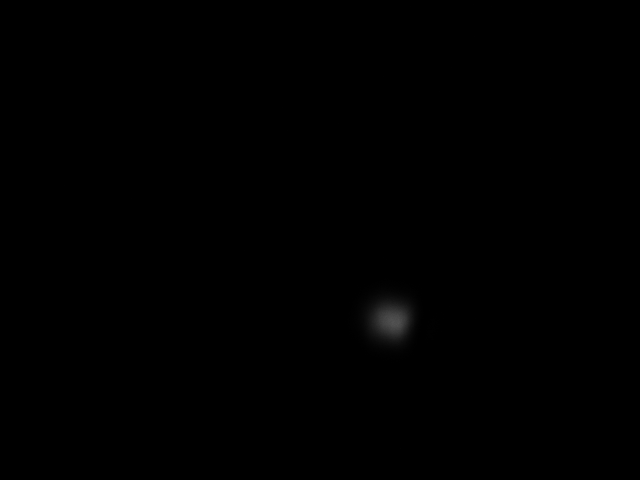
\includegraphics[width=\columnwidth]{kaustik.png}}{figs/kaustik.avi}}
    \only<6>{
      \begin{figure}
        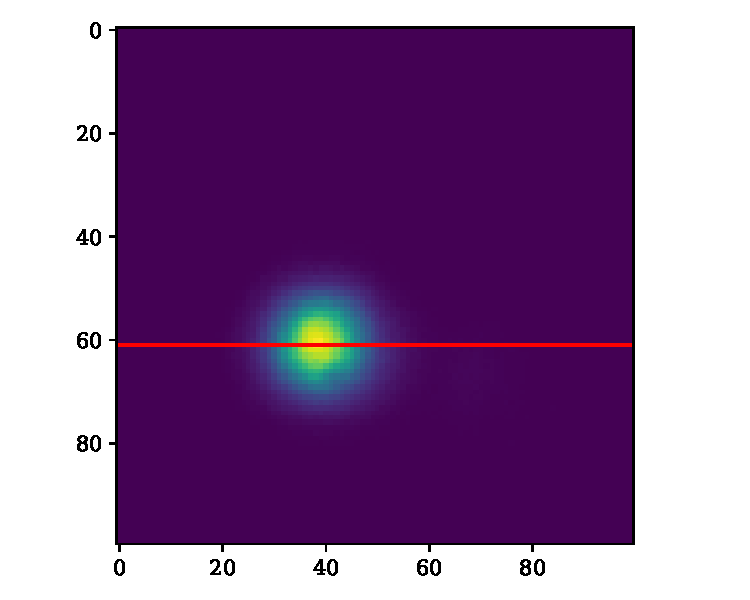
\includegraphics[width=.8\columnwidth]{figs/kaust_red.pdf}
      \end{figure}
    }
    \only<7>{
      \begin{figure}
        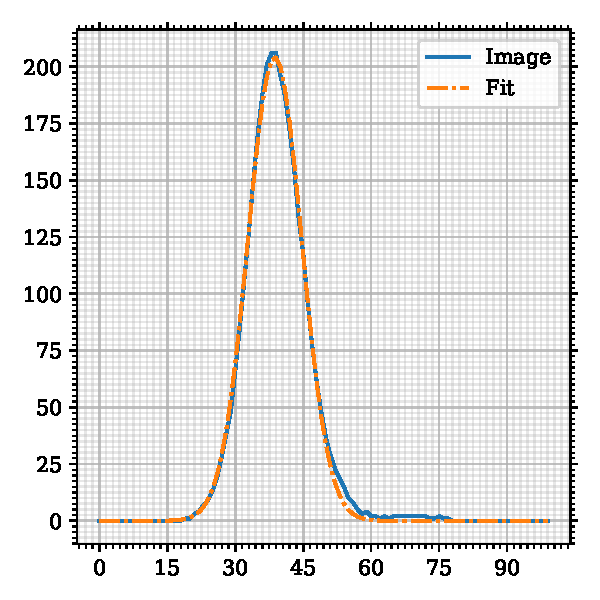
\includegraphics[width=.8\columnwidth]{figs/peakfit.pdf}
      \end{figure}
    }
  \end{columns}
\end{frame}


\begin{frame}
  \begin{figure}[b]\centering
    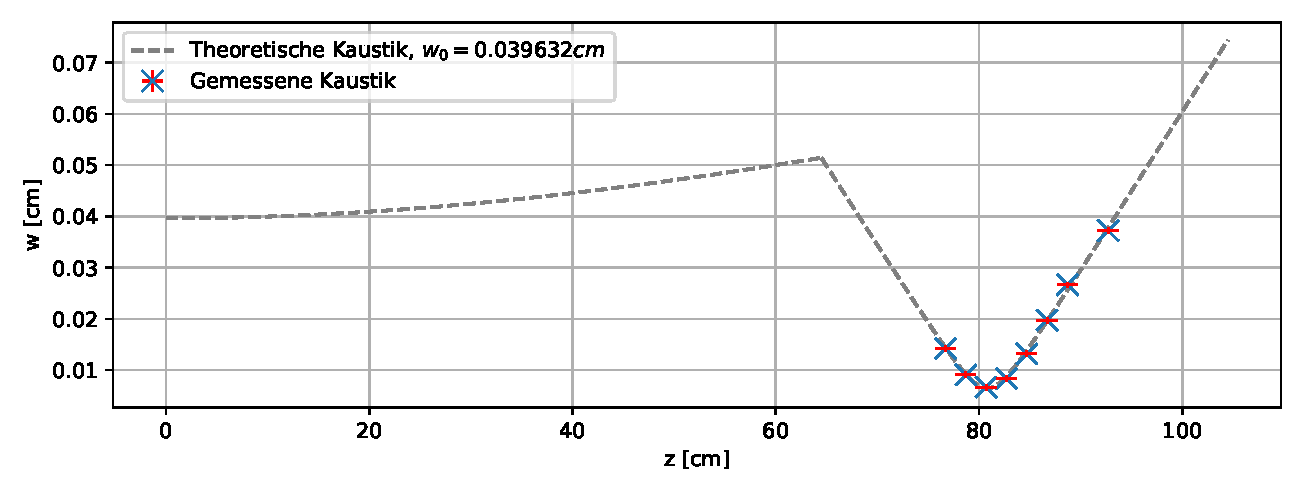
\includegraphics[width=.8\columnwidth]{figs/kaustik.pdf}
  \end{figure}
  \begin{itemize}
  \item<1-> Fit von \(w_0\) (initialer Beamwaist) und einem
    Mess-Offset \(\delta\)
    \begin{align*}
      w_0 & =\SI{396\pm 16}{\micro\meter} \\
      \delta & =\SI{1.2}{cm}
    \end{align*}
  \item<2-> extrem gute \"Ubereinstimmung mit der Theorie \(\implies\)
    verifiziert Matrizenoptik und Gausstrahll\"osung
  \item<3-> theoretischer Wert f\"ur Beamwaist: \SI{284}{\micro\meter}
  \end{itemize}
  \note<1->[item]{w ist 2 sigma, umrechnung noetig}
  \note<2->[item]{artefakt des fits, aber nur 2 param}
  \note<3->[item]{Unbekannte Optik in Kamera, geometrie der Spiegiel
    etc, Rechenfehler}
\end{frame}


\section{Fazit/Quellen}

\begin{frame}{Fazit}
  \begin{itemize}
  \item<1-> erfolgreicher Eigenbau eines Lasers
  \item<2-> gr\"o\ss{}tenteils vern\"unftige Ergebnisse, gute
    \"Ubereinstimmung mit der Theorie
  \item<3-> gro\ss{}er Wissenszuwachs (Matrizenoptik, Gaussstahlen
    etc.)
  \item<4-> toller Betreuer :P (schleim...)
  \end{itemize}
\end{frame}

\begin{frame}[allowframebreaks]{Ausgesuchte Quellen}
  \printbibliography
\end{frame}

% \subsection*{Graveyard}
% \begin{frame}{Crashkurs Matrizenoptik}
%   \begin{itemize}
%   \item<1-> Annahmen: Paraxiale Optik, alle Winkel Klein
%   \item<2-> stelle strahl als 2er Vektor da:
%     \begin{equation}
%       \mqty(d \\ \alpha) \widehat{=} \mqty(\text{Abstand zur Achse} \\
%       \text{Winkel zur Achse})
%     \end{equation}

%   \item<3-> optisches System dargestellt druch Matrix als Produkt der
%     Komponenten:
%     \begin{gather}
%       \label{eq:systmatrix}
%       \mathfrak{M}_{\text{System}}=\mathfrak{M}_{\text{1}}\cdot\ldots\cdot\mathfrak{M}_{n}=\mqty(A
%       & B \\ C & D) \\
%       \mqty(d' \\ \alpha') = \mathfrak{M}_{\text{System}}\cdot\mqty(d
%       \\ \alpha)
%     \end{gather}
%   \end{itemize}
% \end{frame}
% \begin{frame}{Einige Optische Komponenten}
%   \begin{table}[h!]
%     \begin{tabular}{l | c | l}
%       \textbf{Element} & \textbf{Matrix} & \textbf{Parameter} \\
%       \midrule\\
%       \addlinespace[-2ex]
%       freie Ausbreitung & \(\begin{pmatrix}
%         1 & s \\
%         0 & 1
%       \end{pmatrix}\) & Wegl\"ange \(s\) \\
%       \midrule\\
%       \addlinespace[-2ex] d\"unne Linse & \(\begin{pmatrix}
%         1 & 0 \\
%         -1/f & 1
%       \end{pmatrix}\) & Brennweite \(f\) \\
%       \midrule\\
%       \addlinespace[-2ex] sph\"arischer Spiegel & \(\begin{pmatrix}
%         1 & 0 \\
%         -2/R & 1
%       \end{pmatrix}\) & Radius \(R\) \\

%     \end{tabular}
%   \end{table}
% \end{frame}

% \begin{frame}{Gaussstrahlen und Matrizenoptik}
%   \begin{alertblock}{Achtung, High-Level}
%     Sieht komisch aus ist aber so.\note<1->[item]{Urspr\"unge ein
%       wenig erkl\"aren.}
%   \end{alertblock}

%   \begin{itemize}
%   \item<2-> definiere
%     \(\frac{1}{q(z)}=\frac{1}{R(z)}-i\frac{\lambda}{\pi
%       w^2(z)}=a+i\cdot b\) \note<2->[item]{ist exponent der e funktion
%       in mathem. Darstellung Gausstrahl}
%   \item<3-> mit
%     \(\mathfrak{M}_{\text{System}} = \mqty(A & B \\ C & D)\)
%     transformiert sich \(q\) wie folgt:
%     \begin{equation}
%       \label{eq:qtrans}
%       q'=\frac{Aq + B}{Cq+D}
%     \end{equation}
%     \only<4>{
%     \item f\"ur den Beamwaist im vorliegenden Resonator ergibt sich
%       mit \(R\) (Radius Spiegel):\note<5->[item]{param erklaeren}
%       \begin{equation}
%         \label{eq:konfwaist}
%         w_0^4=\qty(\frac{\lambda}{\pi})^2L(R-L)
%       \end{equation}
%     } \only<5>{
%     \item der Beamwaist des Austretenden strahls, verschoben zu Linse
%       fokussiert durch Linse mit Brennweite (A,B,C,D entsprechend
%       Tabelle):
%       \begin{equation}
%         \label{eq:qkaust}
%         b'=b\cdot\frac{AD-CB}{A^2+B^2b^2}
%       \end{equation}
%       \begin{equation}
%         \label{eq:reswaist}
%         w'=\sqrt{\frac{\lambda}{\pi\cdot b'(x)}}
%       \end{equation}
%     }
%   \end{itemize}
% \end{frame}

% \begin{frame}{Zweite Laserbedingung}
%   \begin{itemize}
%   \item<1-> Betrachtung der d\"ampfung des Strahlungsfeldes im Laser
%   \item<2-> Intensität verringert sich pro doppeltem Umlauf um Faktor
%     \(e^{-\kappa}\) \note<2->[item]{Extinktiosfaktor}
%   \item<3-> Verst\"arkung muss gr\"o\ss{}er sein als Verlust
%   \item<4-> mit Wirkungsquerschnitt \note<4->[item]{Wir nehmen an dass
%       sie gilt.}  \(\sigma_{21}=B_{21}\frac{h\cdot\nu}{c}\) ergibt
%     sich:
%     \begin{equation}
%       \label{eq:zwlabe}
%       \tag{zweite Laserbedingung}
%       \sigma_{21}\cdot (N_2-N_1)\cdot 2L \geq \kappa
%     \end{equation}
%   \end{itemize}
% \end{frame}

% \begin{frame}{Resonanz und Modenstruktur}
%   \begin{columns}
%     \column{.5\textwidth} \only<3->{
%       \begin{figure}
%         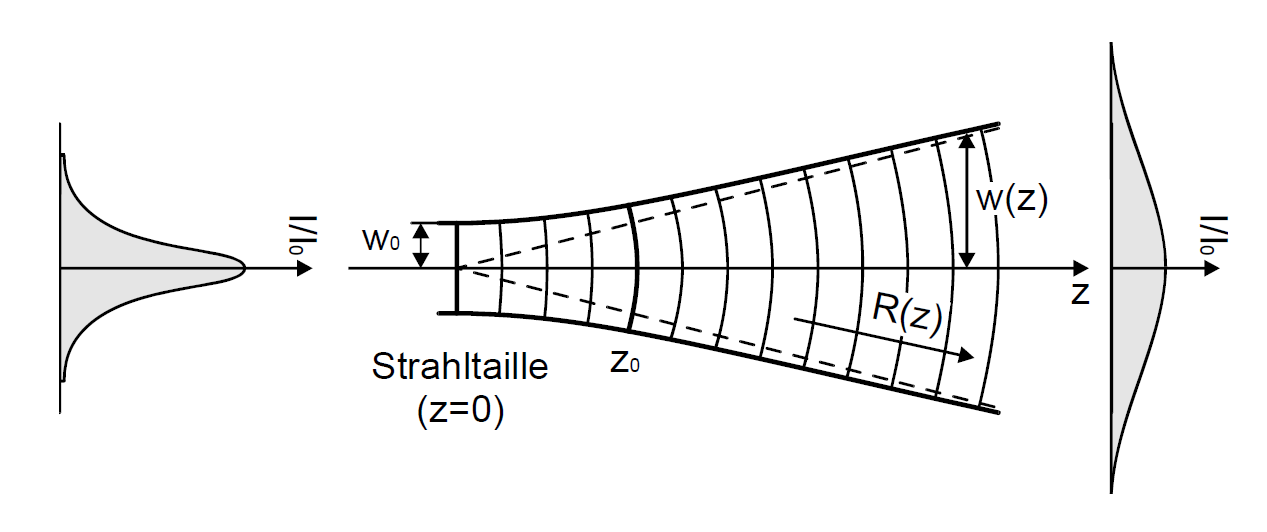
\includegraphics[width=1\columnwidth]{gauss-strahl.png}
%       \end{figure}
%     } \column{.5\textwidth}
%     \begin{itemize}
%     \item<1-> longitudnale Resonanzbedingungg:\note<1->[item]{stehende
%         Welle, in realit\"at nur ein paar moden ausgepraegt,
%         Modenkonkurrenz}
%       \begin{equation}
%         \label{eq:longmodes}
%         L=n\cdot\frac{\lambda}{2} \implies \Delta\nu = \frac{c}{2L}
%       \end{equation}
%     \item<2-> Beschreibung des gesamten Feldes durch paraxiale
%       L\"osung des Maxwell gleichungen \note<2->[item]{Vakuum,
%         anpassen der RB an Spiegel Radien}
%     \item<3-> ergibt als Grundmode sog. \textbf{Gauss-Strahl}
%       (Querschnitt ist Gaussfunktion) \note<3->[item]{h\"ohere Moden
%         weiter aufgeweitet und leicht mit Blenden zu unterdr\"ucken}
%       \only<3>{
%         \begin{itemize}
%         \item charakterisiert durch Strahldicke \(w(z)\), Radius der
%           Wellenfronten \(R(z)\)
%         \item freihe Parameter: Amplitude, Strahltaille \(w(z=0)=w_0\)
%           und Wellenl\"ange
%         \end{itemize}
%       }
%     \item<4-> meist wird eine Polarisation mit einem Brewsterfenster
%       \note<4->[item]{TAFEL} ausgew\"ahlt\note<4->[item]{Auswahl und
%         Verst\"arkung erkl\"aren}
%     \end{itemize}
%   \end{columns}
% \end{frame}

% \begin{frame}{Besetzungsinversion}
%   \begin{itemize}
%   \item<1-> im thermischen Gleichgewicht \"uberwiegt die spontane
%     Emission gegen\"uber der Induzierten \(\implies\) Erzeugung eines
%     Ungleichgewichts durch ``Pumpen'' \note<1->[item]{im folgenden
%       Spontane Emission vernachl\"assigt, erzeugt aber neue Moden,
%       siehe sp\"ater, konzentriert man verst\"arkung auf best. moden
%       \"uberwiegt stim e} und Auswahl bestimmter Moden im optischen
%     Resonator \note<1->[item]{ Negative Temp}
%   \item<2-> Ratengleichung mit \(\rho\) als spektraler Energiedichte,
%     \(B_{21}\) als \"ubergangwarscheilichkeit der
%     stim. Emisson\note<2->[item]{Modell der Einsteinkoeffizienten, als
%       Bedingung der Verst\"arkung} ergibt:
%     \begin{equation}
%       \label{eq:firstlaser}\tag{Erste Laserbedingung}
%       \dv{q}{t}=\rho(\nu)B_{21}(N_2-N_1) \implies
%       N_2>N_1
%     \end{equation}
%     \(\implies\) Besetzungsinversion
%   \item<3-> Besetzungsinversion ist erst mit Vierniveausystem
%     realisierbar (metastabile Zust\"ande halten Grundzustand
%     lehr)\note<3->[item]{sonst grosse Pumpleistung notwendig, 2 da
%       pumpen mit emission konkurriert, 3 da unteres Niveau
%       Grundzustand, vierniveau hat niveau unter unterem laser niv,
%       pumpen an laser\"ubergan vorbei}
%     \note<3->[item]{ZWEITE LB ERW\"AHNEN}
%   \end{itemize}
% \end{frame}

% \begin{frame}
%   \begin{block}{Acronym}
%     \textsc{Light Amplification by Stimulated Emission of Radiation.}
%   \end{block}

%   \pause

%   \begin{block}{Basic Facts}
%     \begin{itemize}
%     \item erster Laser um 1960 von Theodore H. Maiman
%       \begin{itemize}
%       \item bezeichnet als ``L\"osung auf der Suche nach einem
%         Problem''~\cite{2010}
%       \end{itemize}
%     \item kann sehr fokussiertes und koh\"arentes Licht erzeugen
%     \item findet Anwendung in breiten Bereichen der Technik und
%       Wissenschaft
%       \begin{itemize}
%       \item Barcode Scanner, CD-Spieler, Optische
%         Telekommunikationstechnik
%       \item Erzeugung tiefer Temperaturen, Schockwellen, gro\ss{}en
%         Energiedichten, Holographie, Interferometrie,
%         Teilchenbeschleuniger
%       \end{itemize}
%     \end{itemize}
%   \end{block}
% \end{frame}


% \subsection{Modenstruktur und Linienverbreiterung}
% \begin{frame}
%   \begin{itemize}
%   \item<1-> prinzipiell Verst\"arkung von allen Moden, die:
%     \begin{itemize}
%     \item die longitudinale Frequenzbedingungg erf\"ullen
%     \item \"uber der Verlustgrenze liegen \note[item]{unbedingt
%         Konkurrenz erkl\"aren}
%     \end{itemize}
%   \note<1->[item]{nur wenige longitudinale und nicht-Gauss Moden werden
%     verst\"arkt (Konkurrenz, Aufweitung)~\cite[171]{Sigrist2018}}
%   \item<2-> stimulierte Emission akzeptiert aufgrund der
%     sog. \emph{Linienverbreiterung} Frequenzintervalle
%   \item<3-> dadurch Aufweichung von longitudinaler Frequenzbedingung
%   \end{itemize}
% \end{frame}

% \begin{frame}[t]{Mechanismen Linienvebreiterung}
%   \begin{columns}
%     \column{.5\linewidth}
%     \begin{block}{Homogen}
%       \begin{figure}
%         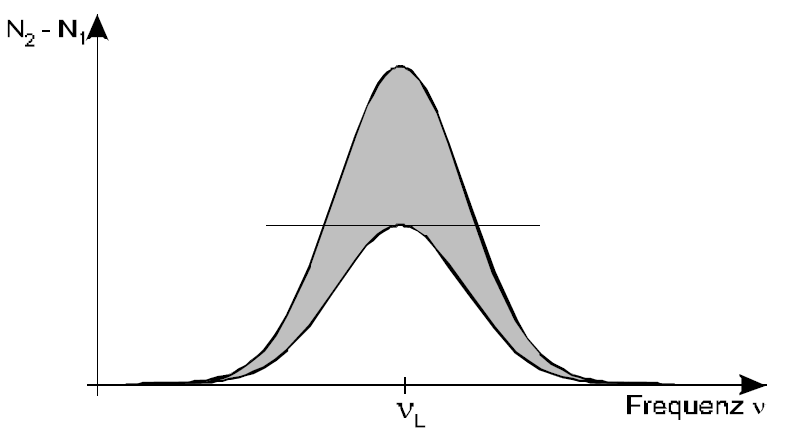
\includegraphics[width=.4\columnwidth]{homogen.png}
%       \end{figure}
%       \begin{itemize}
%       \item<1-> wirkt auf gesamtes aktives Medium
%       \item<2-> Ursachen: Energie-Zeit Unsch\"arfe, strahlungsfreie
%         \"Uberg\"ange, elastische St\"o\ss{}e
%         (Druckverbreiterung)\note<2->[item]{unter anderem}
%       \end{itemize}
%     \end{block}
%     \column{.5\linewidth}
%     \begin{block}{Inhomogen}
%       \begin{figure}
%         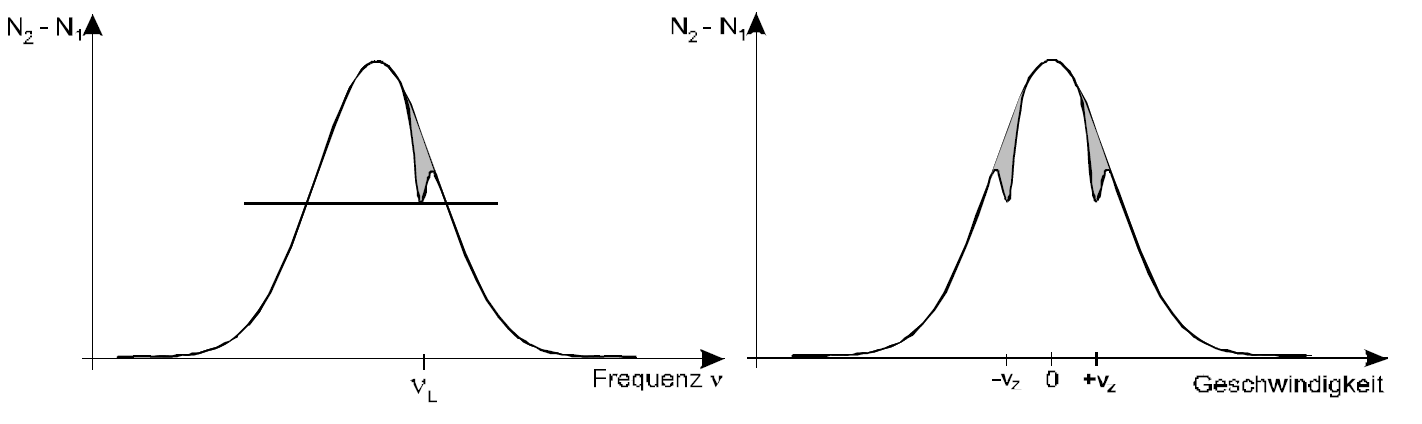
\includegraphics[width=.7\columnwidth]{inhomogen.png}
%       \end{figure}
%       \begin{itemize}
%       \item<1-> wirkt nur auf bestimmte Atomgruppen
%       \item<2-> Ursachen: Dopplereffekt (Dopplerverbreiterung) beim \hne{}-Laser
%         dominant
%       \item<3-> Breite: abh\"angig von der Temperatur

%         \note[item]{kann sog. \emph{Hole-Burning} bewirken:
%           Besetzungsinversion auf bestimmten Atomgruppen abgebaut
%           \(\implies\) stehen nicht mehr f\"ur den Laserprozess zur
%           Verf\"ugung}
%       \end{itemize}
%     \end{block}
%   \end{columns}
% \end{frame}


% \subsection{Messung der Polarisationseigenschaften}
% \begin{frame}
%   \begin{itemize}
%   \item<1-> Einbringen eines Polarisationsfilters in den Strahlengang
%   \item<2-> Messen der Ausgangsleistung bei
%     versch. Polfiltereinstellungen
%     \begin{itemize}
%     \item Messzeit \SI{1}{\minute}
%     \item \(\Delta\phi \approx 1^\circ\)
%     \end{itemize}
%   \end{itemize}
%   \note<1->[item]{Ein wenig zum brewsterfenster}
% \end{frame}

% \begin{frame}
%   \begin{figure}[b]\centering
%     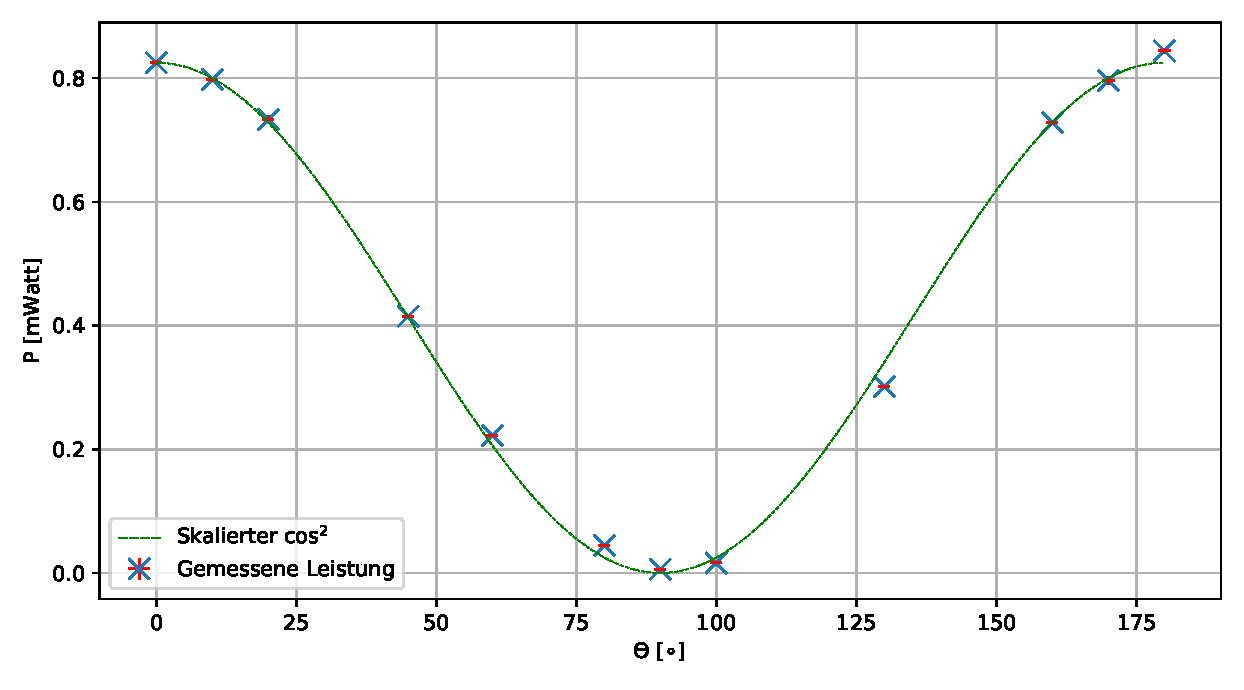
\includegraphics[width=.8\columnwidth]{figs/malus.pdf}
%   \end{figure}
%   \begin{itemize}
%   \item<1-> Theoretische Kurve aus
%     \(I(\Theta)=I_0\cdot \cos^2{\Theta}\)
%   \item<2-> gute Übereinstimmung mit der Theorie \(\implies\) Licht
%     ist linear polarisiert
%   \item<3-> nicht richtig polarisierte Moden werden unterdr\"uckt
%   \end{itemize}
% \end{frame}


% \section{Spektrale Eigenschaften des Lasers}
% \subsection{Fabry-Pérot-Interferometer}
% \label{sec:fpi}
% \begin{frame}
%   \begin{columns}
%     \column{.5\textwidth}
%     \begin{figure}
%       \only<1>{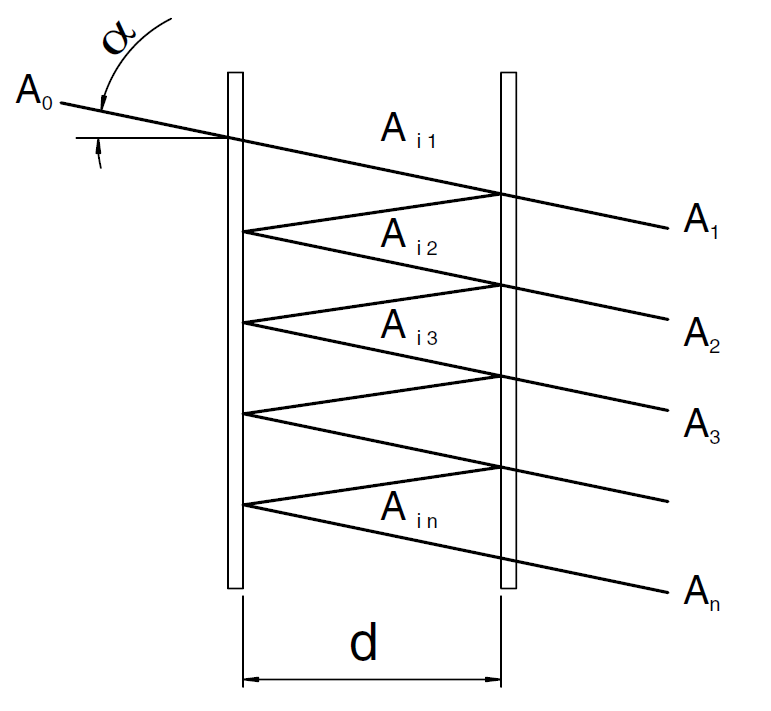
\includegraphics[width=1\columnwidth]{fpiref.png}}
%       \only<2->{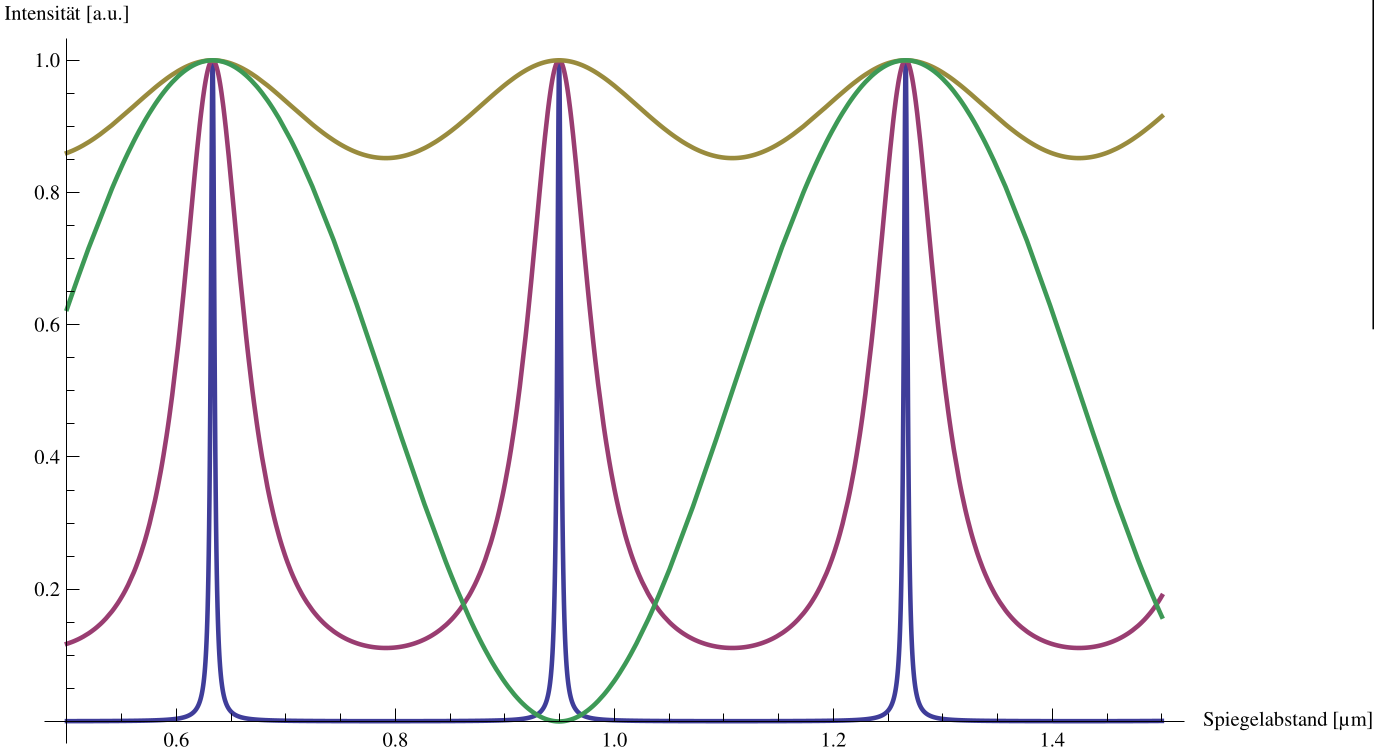
\includegraphics[width=1\columnwidth]{fpitrans.png}}
%     \end{figure}
%     \column{.5\textwidth}
%     \begin{itemize}
%     \item<1-> Vielstrahlinterferenz durch Reflexion zwischen zwei
%       ebenen Spiegeln (Etalon)\note<1->[item]{\textbf{wieder ein Resonator}}
%       \begin{itemize}
%       \item bestimmt durch Abstand \(d\), Reflexionsverm\"ogen \(R\)
%       \end{itemize}
%      \note<2->[item]{nur f\"ur \(d=n\cdot\frac{\lambda}{2}\)
%       \SI{100}{\percent} Transmission}
%     \item<3-> sehr scharfe Maxima \(\implies\) hohe Aufl\"osung
%     \end{itemize}
%   \end{columns}
% \end{frame}

% \begin{frame}
%   \begin{columns}
%     \column{.5\textwidth}
%     \begin{figure}
%       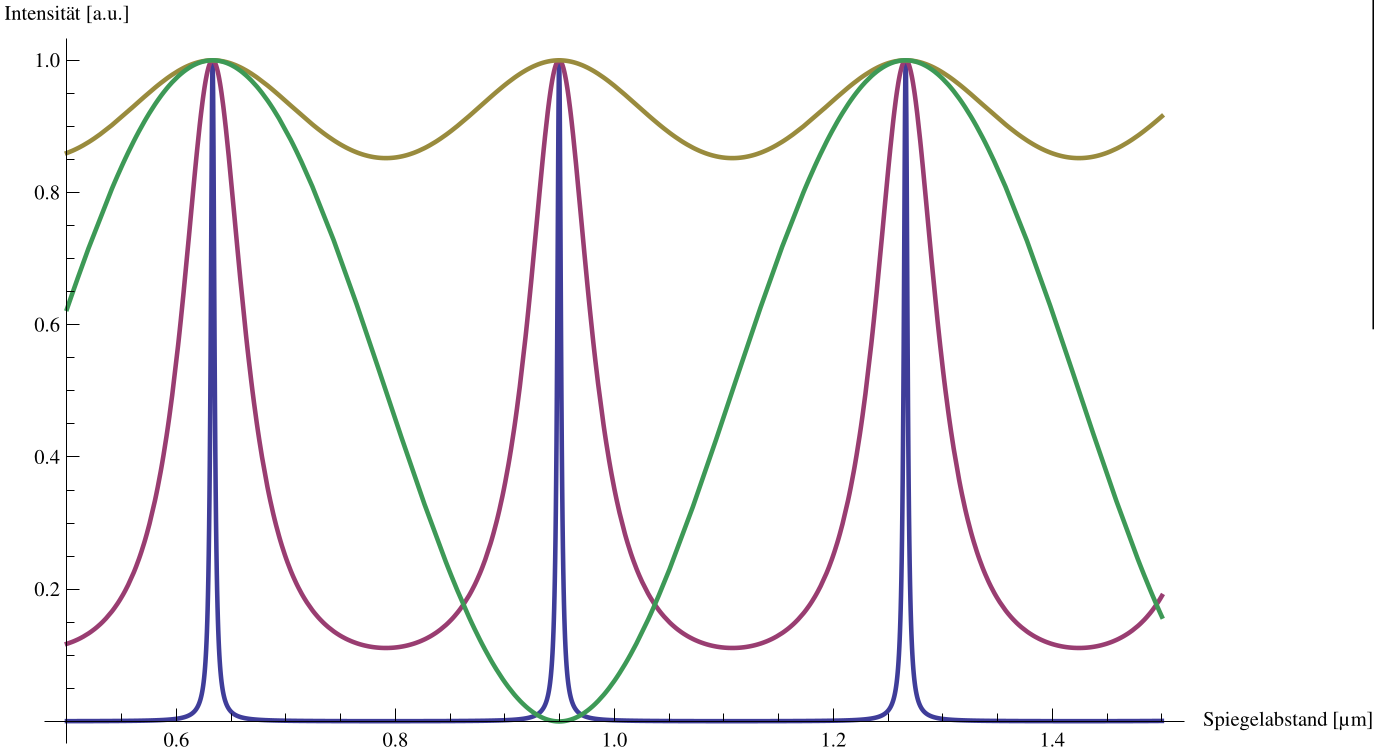
\includegraphics[width=1\columnwidth]{fpitrans.png}
%     \end{figure}
%     \column{.5\textwidth}
%     \begin{block}{Charakterisierung eines FPI}
%       \begin{description}
%       \item<1->[Free Spectral Range (FSR)] Abstand der transm. Maxima,
%         genutzt zur Kalibrierung \note<1->[item]{Breite
%           Unterscheidbarer Frequenzen, genutzt zur }
%         \begin{equation}
%           \label{eq:fsr}
%           \text{FSR} = \frac{c}{2\cdot d} = \delta\nu
%         \end{equation}
%       \item<2->[Finesse] Quotient aus FSR und Halbwertsbreite
%         \note<2->[item]{es sollte \(R\rightarrow 1\)}
%         \begin{equation}
%           \label{eq:finesse}
%           \mathfrak{F} = \frac{\pi\sqrt{R}}{1-R}
%         \end{equation}
%       \end{description}
%     \end{block}
%   \end{columns}
% \end{frame}

% \section{Durchf\"uhrung und Ergebnisse}
% \label{sec:durchf}


% \subsection{Messung des Spektrums mit dem Faserspektrometer}
% \begin{frame}
%   \begin{figure}
%     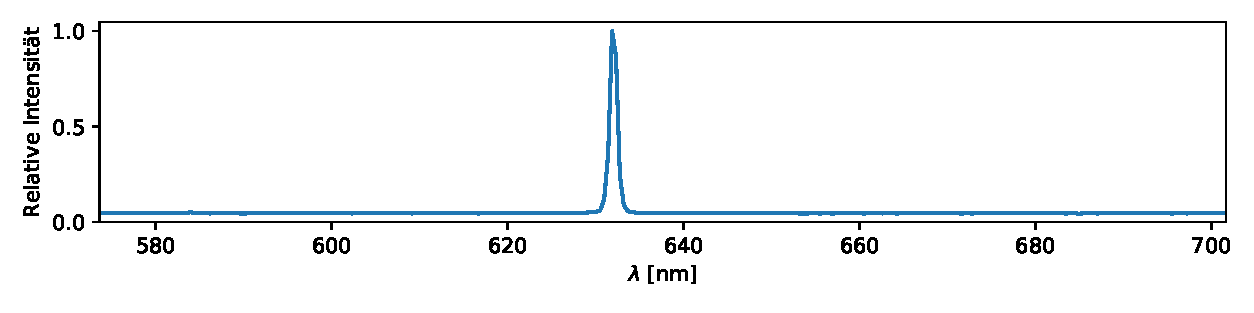
\includegraphics[width=1\columnwidth]{figs/faserspek.pdf}
%   \end{figure}
%   \begin{itemize}
%   \item<1-> Aufnahme des Spektrums des Lasers mit einem
%     Faserspektrometer (\textsc{Ocean Optics HR+C1743})
%     \begin{itemize}
%     \item erlaubt absolute Frequenzessung
%     \end{itemize}
%   \item<2-> gro\ss{}er Peak bei \(\lambda_0=\SI{631.9}{\nano\meter}\)
%     \begin{itemize}
%     \item<3-> bei \SI{632.8}{\nano\meter} deutlich unter der
%       Peakh\"ohe \(\implies\) Spektrometer schlecht kalibriert
%       \note<3->[item]{spricht gegen bias als statistik da peak
%         symetr.}
%     \end{itemize}
%   \end{itemize}
% \end{frame}

% \begin{frame}
%   \begin{itemize}
%   \item<1-> Abstand der Messpunkte
%     \(\Delta\lambda=\SI{.5}{\nano\meter}\) \uncover<2->{ \\
%       \(\implies\) bestm\"ogliche Aufl\"osung:
%       \begin{equation}
%         \Delta\nu=c\cdot\frac{\Delta\lambda}{\lambda_0^2}=\SI{3.30e11}{\hertz}
%       \end{equation}}
%   \item<3-> aus \(L=\SI{80+-.5}{\centi\meter}\) ergibt sich
%     \note<3->[item]{Ungenauigkeit war sehr klein}
%     \begin{equation}
%       \label{eq:moda}
%       \delta\nu = \SI{1.87e8}{\hertz} < \Delta\nu
%     \end{equation}
%     \uncover<4->{ \(\implies\) einzelne Moden k\"onnen nicht
%       aufgel\"ost werden }
%   \end{itemize}
% \end{frame}

% \subsection{Messung von Spektra mit dem FPI}
% \begin{frame}
%   \begin{itemize}
%   \item<1-> wiederum Justage des Strahlengangs durch R\"uckreflexe
%   \item<2-> Bestimmung des Abstandes der Spiegel zu
%     \begin{equation*}
%       d=\SI{7.50+-0.25}{\centi\meter}
%     \end{equation*}
%     \only<3->{
%       \begin{alertblock}{Mehrfachuml\"aufe}
%         Falls der Strahl nicht exakt senkrecht auf die Spiegel trifft
%         kommt es zu Mehrfachuml\"aufen und einer Verdopplung des
%         Wegunterschiedes.
%       \end{alertblock}}
%   \item<4-> Aufnahme des Spektrums des kommerziellen und des offenen
%     Lasers durch Modulation (S\"agezahn) des Spiegelabstandes
%   \end{itemize}
%   \note<2->[item]{Ungenauigkeit gesch\"atzt} \note<3->[item]{da
%     konfokales fpi,
%     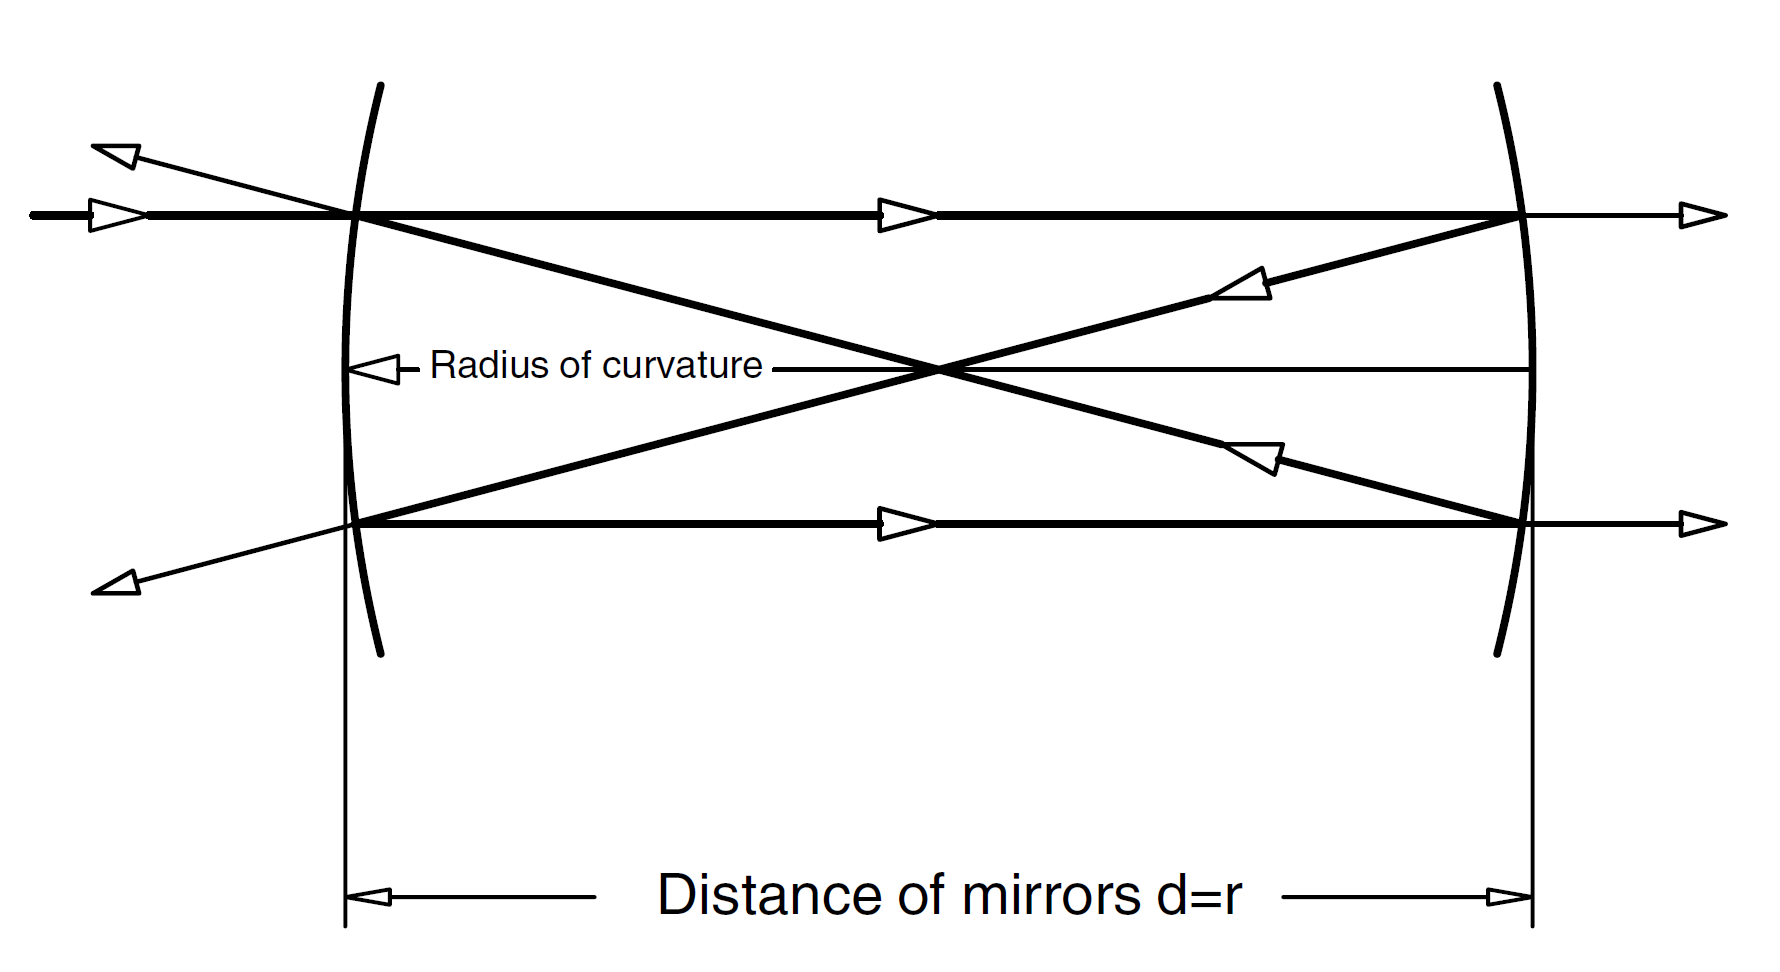
\includegraphics[width=.4\columnwidth]{mehrfach.png}}
% \end{frame}

% \begin{frame}{Kalibrierung der Zeitachse (kommerzieller Laser)}
%   \begin{figure}
%     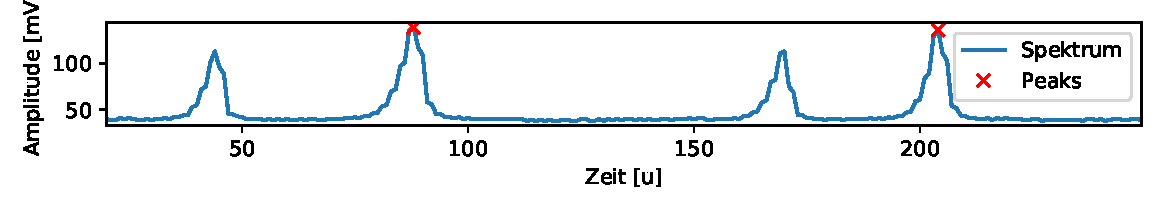
\includegraphics[width=1\columnwidth]{figs/fsrkalib.pdf}
%   \end{figure}
%   \begin{itemize}
%   \item<1-> der FSR berechnet sich aus der L\"ange des FPI zu
%     \begin{equation}
%       \label{eq:realfsr}
%       \text{FSR} = \SI{2.00+-0.07}{\giga\hertz}
%     \end{equation}
%   \item<2-> Kalibrierung der willk\"urlichen Zeiteinheit \(u\)
%     (\(\Delta t = \SI{1}{u}\), 1 Digit) durch Abstands der Peaks
%     \begin{eqnarray}
%       \label{eq:unithertz}
%       \si{u} = \frac{\text{FSR}}{t_2-t_1} =\SI{.172}{\mega\hertz} \\
%       \Delta\si{u}  = \sqrt{\qty(\frac{\Delta\text{FSR}}{x_2-x_1})^2 +
%       2\cdot\qty(\frac{\text{FSR}}{(x_2-x_1)^2}\Delta t)^2}  & = \SI{.07}{\mega\hertz}
%     \end{eqnarray}
%   \end{itemize}
% \end{frame}

% \begin{frame}{Bestimmung der Finesse}
%   \begin{figure}
%     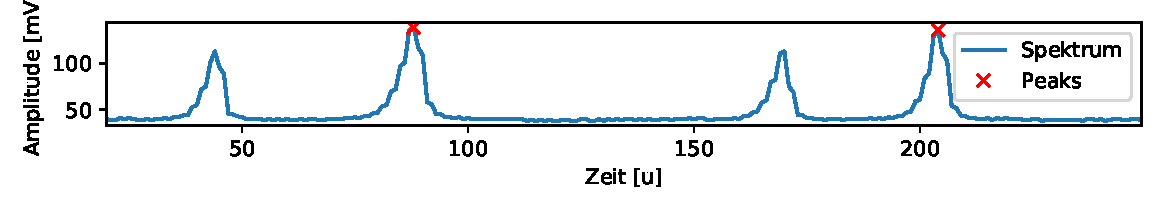
\includegraphics[width=1\columnwidth]{figs/fsrkalib.pdf}
%   \end{figure}
%   \begin{itemize}
%   \item<2-> Bestimmung der Finesse durch Mittlung \"uber 4 Peaks

%     \begin{align}
%       \label{eq:fwhmlaser}
%       \overline{\text{FWHM}} =&\; \SI{4.72}{u} = \SI{81\pm
%                                 6}{\mega\hertz} \\
%       \mathfrak{F} =& \frac{\text{FSR}}{\text{FWHM}}=\SI{24.6\pm 2.0}{}
%     \end{align}
%   \item<3-> nicht \"uberragend (typischerweise \(> 50\) bei kleinem
%     Strahldurchmesser\cite{HENDOW1997343}) aber ausreichend zur
%     Aufl\"osung individueller Moden
%   \end{itemize}
% \end{frame}

% \begin{frame}{Modenstruktur des kommerziellen Lasers}
%   \begin{figure}[b]\centering
%     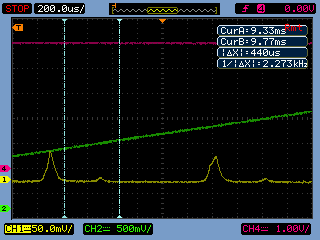
\includegraphics[width=.3\columnwidth]{pol1.png}
%     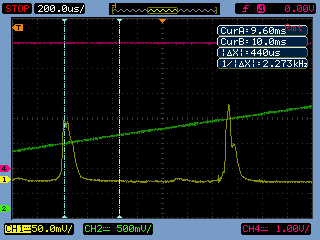
\includegraphics[width=.3\columnwidth]{pol2.png}
%     \caption[Gauss]{Spektrum des kommerziellen \hne{}s f\"ur zwei
%       orthogonale Polarisationsrichtungen}
%   \end{figure}

%   \begin{itemize}
%   \item beide sichtbaren Moden genau orthogonal polarisiert
%   \end{itemize}
% \end{frame}

% \begin{frame}{Modenstruktur des kommerziellen Lasers}
%   \begin{figure}[b]\centering
%     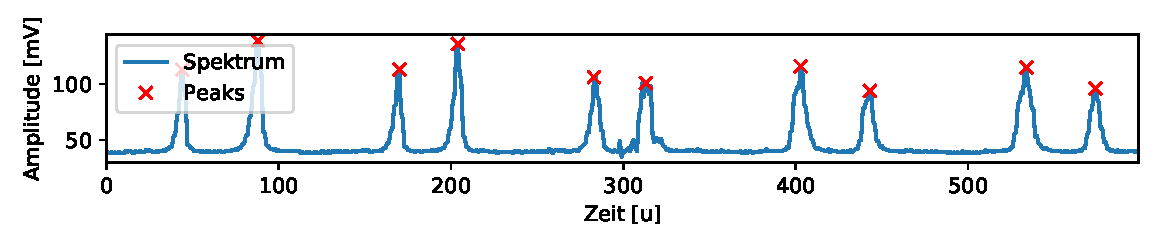
\includegraphics[width=1\columnwidth]{figs/komm_all_peaks.pdf}
%   \end{figure}

%   \begin{itemize}
%   \item<1-> Bestimmung des Modenabstandes durch Mittlung \"uber alle
%     \(5\) sichtbaren Gruppen
%     \begin{equation}
%       \label{eq:modeabstkom}
%       \overline{\delta\nu_k}=\SI{37.6\pm 2.2}{u}=\SI{650\pm 40}{\mega\hertz}
%     \end{equation}
%   \item<2-> daraus berechnet sich die Resonatorlänge
%     \begin{align}
%       L_k =& c/(2\cdot \delta\nu_k = \SI{23.1\pm 1.6}{\centi\meter}
%     \end{align}
%     \begin{itemize}
%     \item<3-> erscheint plausibel
%     \item<3-> Pr\"azision der L\"ange vergleichbar mit vorherigen
%       Ergebnissen
%     \end{itemize}
%   \end{itemize}
%   \note<1->[item]{intersannter weise: Umkehrung der Peakh\"ohen}
%   \note<1->[item]{ungenauigkeit aus Statistik}
% \end{frame}

% \begin{frame}{Modenstruktur des offenen Lasers}
%   \begin{columns}
%     \column{.5\textwidth}
%     \begin{figure}
%       \only<1>{
%         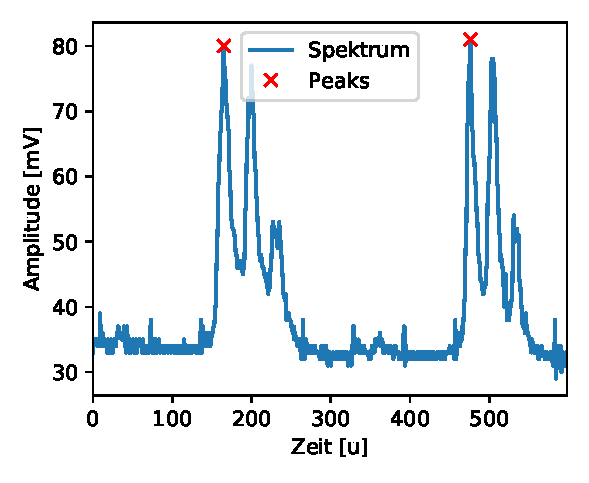
\includegraphics[width=1\columnwidth]{figs/off_80.pdf}}
%       \only<2>{
%         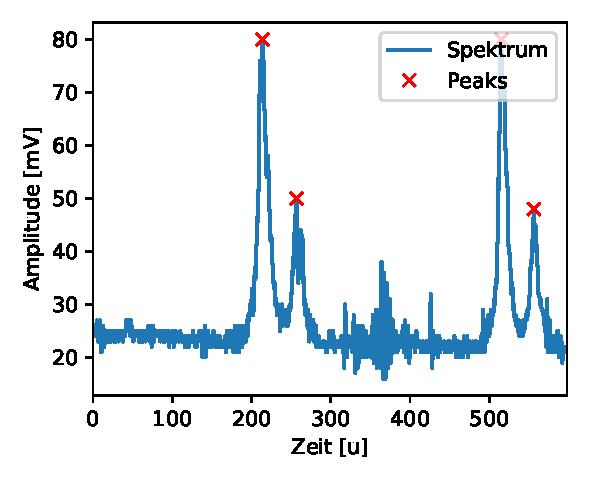
\includegraphics[width=1\columnwidth]{figs/off_60.pdf}}
%     \end{figure}
%     \column{.5\textwidth}
%     \begin{itemize}
%     \item<1-> analoge Bestimmung des Modenabstandes
%     \item<2-> Anzahl der Peaks f\"ur \(L=\SI{60}{\centi\meter}\) sehr
%       gering
%     \end{itemize}
%   \end{columns}
% \end{frame}
% \begin{frame}{Modenstruktur des offenen Lasers}
%   \begin{table}
%     \begin{tabular}{SSS}
%       \toprule
%       {\(L\) [\si{\centi\meter}]} & {\(\delta\nu\) Theorie [\si{\mega\hertz}]} & {\(\delta\nu\) experimentell [\si{\mega\hertz}]}\\
%       \midrule
%       80 & 187.4\pm 1.2 & 201\pm 14 \\
%       60 & 249.8\pm 2.1 & 279\pm 11 \\
%       \bottomrule
%     \end{tabular}
%   \end{table}
%   \begin{itemize}
%   \item<1-> akzeptable \"Ubereinstimmung mit der Theorie \(\implies\)
%     keine unaufgel\"oste Mode dazwischen
%   \item<2-> bei \(L=\SI{60}{\centi\meter}\) ist die Abweichung
%     untersch\"atzt
%   \end{itemize}
% \end{frame}

% \begin{frame}{Betrachtung der Linienverbreiterung}
%   \begin{columns}
%     \column{.5\textwidth}
%     \begin{figure}
%       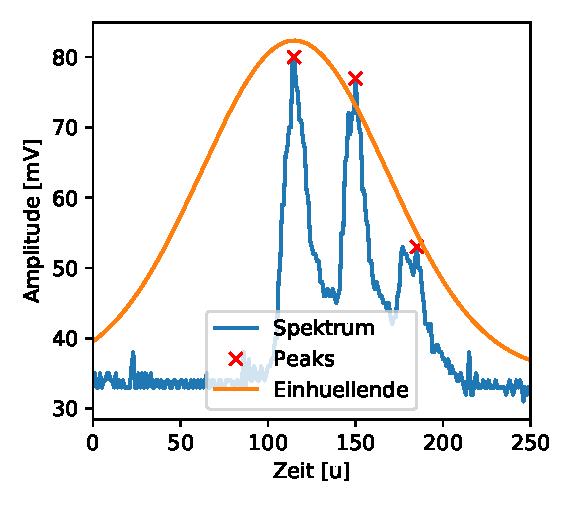
\includegraphics[width=1\columnwidth]{figs/verbr_fit.pdf}
%     \end{figure}
%     \column{.5\textwidth}
%     \begin{itemize}
%     \item<1-> Dopplerverbreitung ist dominant
%     \item<2-> Einh\"ullende des Modenspektrums sollte Gausskurve
%       entsprechen \(\implies\) Bestimmung der Temperatur m\"oglich
%     \item<3-> Fit symmetrisch angesetzt, Amplitude und Breite als freie
%       Parameter
%     \end{itemize}
%   \end{columns}
% \end{frame}

% \begin{frame}{Betrachtung der Linienverbreiterung}
%   \(m=\SI{3.35092e-26}{\kg}\)~\cite{IUPAC2013} und
%   \(\nu_0=\SI{473.755}{\tera\hertz}\) ~\cite[226]{Sigrist2018}
%   \begin{align}
%     \sigma_{\text{Doppler}} & = \nu_0\qty(\frac{kT}{mc^2})^{1/2} \\
%     \sigma & = \SI{53\pm 20}{u} = \SI{340\pm 130}{\mega\hertz} \\
%     T & = \qty(\frac{\sigma\cdot c}{\nu_0})^2\cdot \frac{m}{k_B}=\SI{110\pm 90}{\kelvin}
%   \end{align}
%   \begin{itemize}
%   \item<1-> Unsicherheit von \(\sigma\) abesch\"atzt
%   \item<2-> Temperatur viel zu gering (f\"ur realistische Temperaturen
%     doppelte Breite)
%     \begin{itemize}
%     \item \(3\) Peaks und \(2\) freie Parameter lassen keinen genauen
%       fit zu
%     \end{itemize}
%   \end{itemize}
%   \note<1->[item]{\(\sigma\) \textbf{Fit Param}} \note<2->[item]{da
%     andere Mechanismen vernachl. eher zu hohe temp erwartet!}
% \end{frame}


\end{document}
